\infolevone{\chapter{Hall C Spectrometers}\label{chap:spectrometers}}

\graphicspath{{spectrometers/figs/}}
\renewcommand{\dirfig}[0]{spectrometers/figs}
\renewcommand{\dircur}[0]{spectrometers}

% TODO:
%  Add a bit more detail about detectors in the HMS hut
%  Table of SHMS performance specifications in SHMS section
%  HMS window details in ``Vacuum Windows in Hall C'' table
% Check the statement:
%    The HMS entrance window is located near the pivot and has a center-to-center
%   bolt hole diameter of $10.5$ inches.

\infoleveqnull{\section{Hall C Spectrometers}}
\infolevone{
%\section{Introduction}

	The two magnetic spectrometers in Hall~C are designed to perform
high resolution and high accuracy nuclear physics experiments.  These
spectrometers transport and detect charged particles that are scattered or produced
in beam-target interactions.
\ifdefined\SHMSMAGNETSOSP
In this document we discuss the features and safe operation of
the Super High Momentum Spectrometer, or SHMS.
After this introduction and overview of the SHMS, the
SHMS (and the legacy HMS - High Momentum Spectrometer)
are discussed together as a series of subsystems.
This document
\else
In this chapter
we discuss the features and safe operation of these spectrometers,
the High Momentum Spectrometer, or HMS,
and Super High Momentum Spectrometer, or SHMS.
These spectrometers
share many common features.  After this
introduction and overviews of the individual spectrometers, the
spectrometers are discussed together as a series of subsystems.
This chapter covers the ``mechanical'' subsystems of the spectrometers.
This chapter
\fi
covers the ``mechanical'' subsystems of the spectrometers.
The detector packages and
shield houses are discussed in
\ifdefined\SHMSMAGNETSOSP
Chapter 5 of the Hall C Standard Equipment Manual~\cite{HallCosp}.
\else
Chapter~\ref{chap:detectors}.
\fi

\ifdefined\SHMSMAGNETSOSP
The SHMS is
\else
Both the HMS and the SHMS are
\fi
designed around a series of superconducting magnets,
including quadrupoles and dipoles, followed by a set of particle detectors.  The first
magnet on the SHMS is a horizontal-bending (HB) dipole that bends particles
away from the beam-line.
\ifdefined\SHMSMAGNETSOSP\else
The HMS does not have a horizontal bender.
\fi
The primary purpose of the quadrupole magnets is to increase the flux of
charged particles entering the main dipole magnets and to focus the orbits of the
charged particles into the detector huts.
The dipole magnets deflect charged particles vertically
as they enter the detector huts. Some of the detectors measure the amount of deflection
so that we may
determine the momentum of each particle. Other detectors provide accurate timing
to trigger the readout of all detector data, or they measure a particle's speed
or total energy so that we can determine its mass.

\ifdefined\SHMSMAGNETSOSP
The SHMS
\else
Each spectrometer
\fi
is built on a rotatable support structure or ``carriage".
These ride on steel
wheels and rails and rotate around the pivot. Experiments using the HMS or
SHMS place their experimental targets along the beamline above the pivot.
The support structures carry the weight of the magnets and detectors, and keep
them aligned to one-another and pointed at the target. On the SHMS, the shield
house and all of the
other spectrometer equipment are also carried by the support structure.
\ifdefined\SHMSMAGNETSOSP\else
The
HMS has a separate carriage that supports the weight of the shield house.
\fi

During beam operations a many particles are scattered and
produced in the target. A few of these enter one of the spectrometers. Most of
them go forward at small angles and are stopped in the beam dump. The
remainder, scattered over a wide range of angles,  interact with the beam pipe,
the air, nearby structures, etc., and
constitute background radiation that would overwhelm the detectors.
The shield houses have thick walls that are designed to reduce the amount of
radiation that gets inside. Both spectrometers use
concrete and lead lining on the walls as shielding. On
the SHMS, two custom types of concrete improve the neutron stopping power
of the walls by
adding boron (in the form of boron-carbide) or extra hydrogen (recycled
plastic chips). Each shield house has a room that surrounds the detectors.
The SHMS has a second room, shielded from the first, that protects the
electronics of the DAQ system and the magnet control systems.

%Each spectrometer includes a shield house which contain the particle
%detector packages.  In the case of the SHMS, this shield house (and a separate
%shield house for electronics) are part of the carriage structure.  In
%the case of the HMS, the detector shield house is a separate
%structure, coupled to the carriage by a ``push bar'' on the ``pasta fork''.
%The ``pasta fork" is the name given to the steel piece that protrudes
%from the back of the carriage. The detector frame is supported on the
%``pasta fork." This insures that the detectors do not move relative
%to the magnetic elements.

\infolevone{
\section{The HMS Detector Package and Shield House }

All the detectors are in the shield house (also referred to as the detector hut,
located at the top of the
rear set of stairs). The shield house has one wall which is removable
in order to gain completely free access to the detectors. The removal
of this wall is rarely needed as there is a door that provides access
to the hut and there is adequate room inside the hut for most activities.
Essentially, the only activities that require the removal of the hut
wall are the installation or removal of an entire detector. The
hut wall may only be removed by Hall~C approved, and trained crane
operators and requires
several people.  Walter Kellner, the Hall~C work coordinator,
must be contacted if the hut wall needs to be removed.

\subsection{HMS Shield House Door}
The HMS shield house and detectors are accessed through a 15 ton
door. This door is moved by energizing the motor attached to it.
Once you have it open as wide as you need, it is suggested that you
use the rubber block provided to chock the door in the open
position. It does tend to drift closed if not restrained. If you find
yourself inside the shield house with the door closed, there are
pushbutton controls inside which you can use to open it (see below).

An interlock prevents access to the HMS detector hut unless the safety
shutter inside the hut has been moved to its `down' position, such
that it covers the vacuum window. This is to prevent people from
accidentally touching the large vacuum window. The door cannot be
opened unless the shutter is already inserted. To prevent the door
from drifting open on its own, a magnetic lock holds it in the closed
position. This lock is de-energized when the OPEN control button is
pressed.

The door is opened or closed by activating the motor attached to its
hinges. The control panel for the door is mounted on the yellow post
(Fig.~\ref{fig:hmsdoorcontrol}) behind
and to your right as you stand in front of the door. A duplicate set
of controls is inside the shield house, to the right of the
door. Press and hold the button marked OPEN and the door will be
slowly opened. Press CLOSE to move the door towards the closed
position. Remember that the door will continue to move after you
release the button because of its inertia. It takes about two minutes
to fully open the door or to close it from the fully opened
position. When closing the door, make certain to keep CLOSE pressed
until the magnetic lock near the top of the door engages.

\begin{figure}
\begin{center}
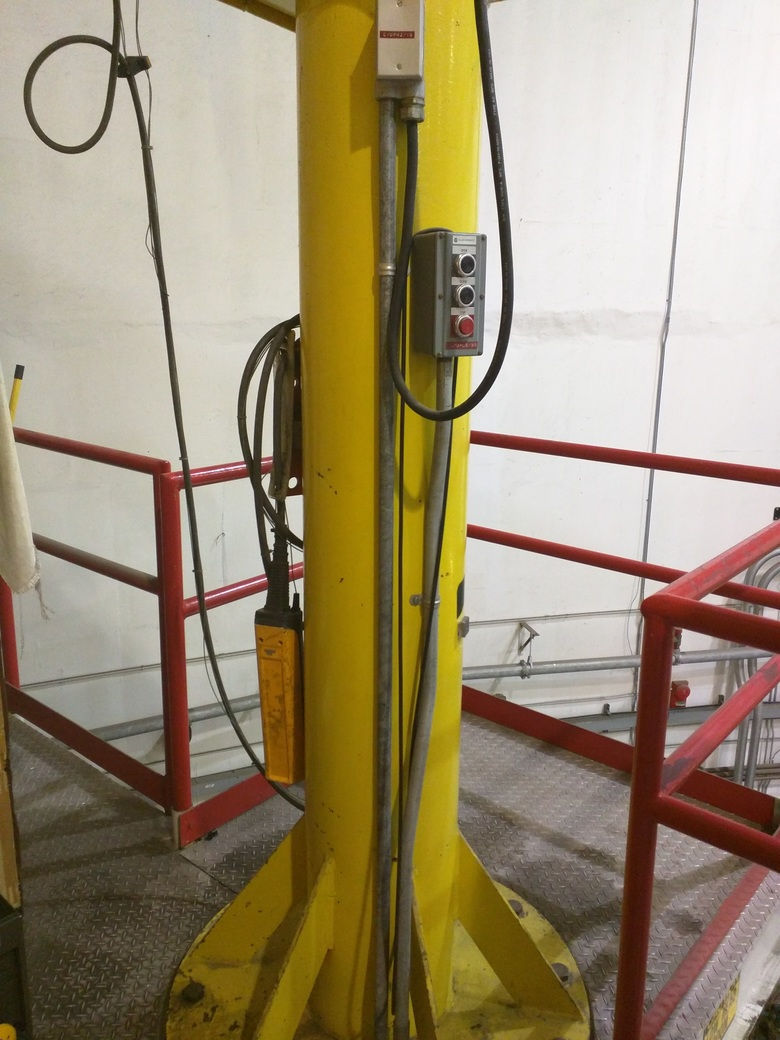
\includegraphics[width=4in]{hmsdoor-control.jpg}
\caption{\label{fig:hmsdoorcontrol}HMS door control buttons.
}
\end{center}
\end{figure}

\subsection{HMS Vacuum Window Shutter}
The HMS vacuum volume extends from near the scattering chamber,
through the three quadrupoles and the dipole, up to the thin aluminum
vacuum window just upstream of the first HMS drift chamber. Because of
the considerable stored energy in such a large vacuum volume, it is
necessary to protect personnel working in the HMS shield house from
the possibiliity of a catastrophic failure of this vacuum.  See
Fig.~\ref{fig:hmsshutter}.

\begin{figure}
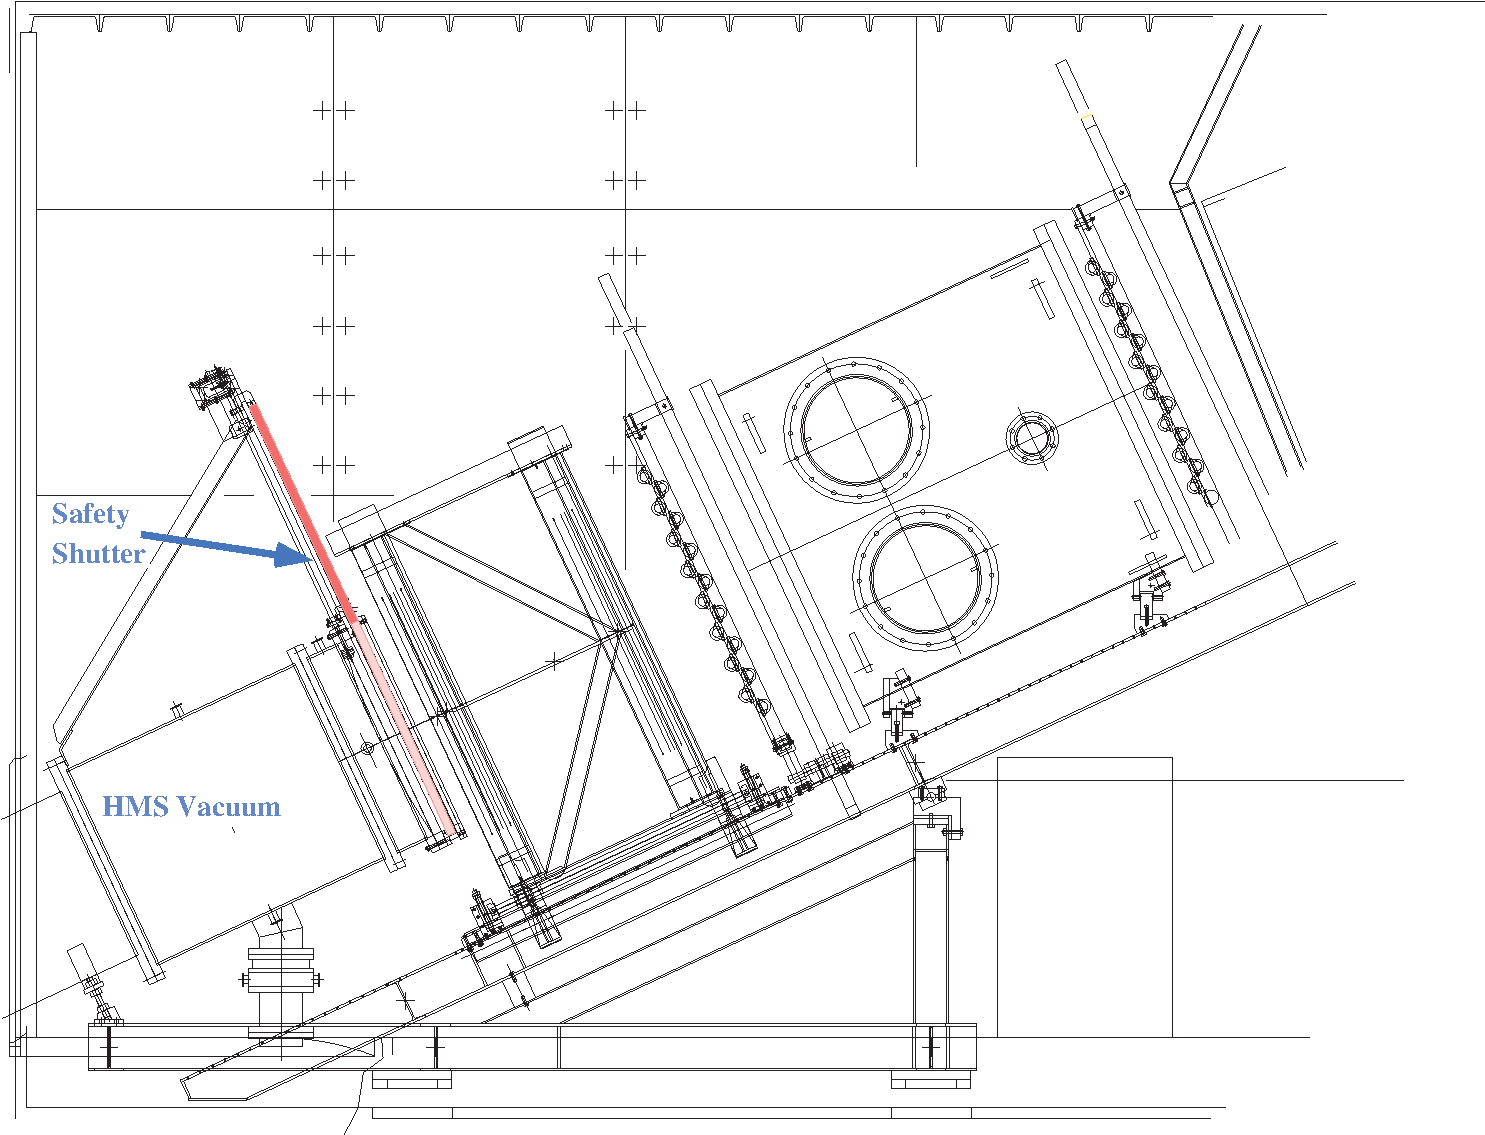
\includegraphics[width=5in]{hms-shutter.pdf}
\caption{\label{fig:hmsshutter}The HMS vacuum window in the HMS spectrometer hut.
}
\end{figure}

Protection is provided by a 1 inch thick aluminum plate which covers
the large vacuum window in the HMS shield house. This plate slides up
and down in an assembly which is atqtached to the end of the vacuum
vessel. Movement of the shutter is managed by a motor which is
controlled from a control box on the outside of the shield house, on
the left side of the door.

An interlock prevents access to the HMS detector hut unless the safety shutter has been moved to its `down' position, such that it covers the vacuum window. This is to prevent people from accidentally touching the large vacuum window, or suffering hearing loss should there be a catastrophic failure of the window. The shutter cannot be retracted unless the door is closed. The door cannot be opened unless the shutter is already inserted.

\subsubsection{Shutter Operation}

To close the shutter, press (and hold for a few seconds) the button
labeled ``DOWN'' on the shutter control box. This will start insertion
of the shutter. After a few seconds the light indicating ``OUT'' will
turn off. It takes about two minutes for the shutter to move into
place. When it does, the light labeled ``IN'' will glow. This
indicates that the shutter is inserted and the door may be opened.  To
open (i.e. raise the shutter, after the HMS shield house door has been
fully closed, press the button labeled ``UP'' and hold it for a few
seconds. The ``IN'' light will dim as the shutter moves away from the
fully inserted position. Full retraction takes about two minutes. When
the shutter is fully retracted, the ``OUT'' light will glow.

Usually the shutter is retracted by MCC operators after they have
swept the interior of the HMS shield house and closed the
door. Experimenters should watch the operators, using the hall survey
TV cameras, to make certain that they complete this step during any
sweep of the hall. If the operators complete the sweep of the hall
without opening the shutter, you will have to make a controlled access
and open the shutter yourself.

If you enter the HMS shield house during Controlled Access, you are
responsible for closing the door and raising the shutter yourself.

``IN'' and ``OUT'' shutter status lights are located both on the
shutter control box and on the top left panel of the Counting House
main console. You can check the status of the shutter from the
Counting House via these lights.



\subsection{Drift Chambers}
The first detectors encountered by particles passing through the HMS
are a pair of drift chambers.  These chambers
provide accurate measurements of the particles
position and angles in the detector hut. This information can be combined
with a knowledge of the spectrometer optics to infer the trajectory of the
particles at the target.

Two sets of drift chambers will be available for the HMS.  The
original set of chambers, described below
(Section~\ref{sec:legacydriftchambers} and new set of chambers of
design very similar to the drift chambers in the SHMS.

Independent of type of chamber, the old and new style chambers are
instrumented in a similar fashion.

The chambers have field shaping wires (and in the case of the new
drift chambers, foils on each side of each sense wire plane) that are
operated at negative high voltage supplied by CAEN high voltage, low
current, power supplies located in the electronics room of the
counting house.  The high voltage can be controlled through a GUI on
the console computers as described in section~\ref{sec:highvoltage}.

Each anode/sense wire has its own electronic readout through
Nanometrics preamplifier/discriminator cards or LeCroy Corporation LRS
2735DC cards which are interchangeable with the Nanometrics cards.
The discriminator outputs from the cards, each of which instruments 16
sense wires are connected to CAEN V1190 multi-hit TDCs located in the
SHMS electronics hut.
The discriminator cards are powered by +5V and -5V Acopian power
supplies that are
located in the HMS hut.  In total, several 10s of amps of both positive
and negative voltage current are supplied.  The supplies are not
computer controlled.

The thresholds of the discriminators are held by a third set of supplies
which are located upstairs in the counting house. This control
is in the left side of the far left hand set of blue racks (near the disk drives) in the
electronics bay of the Hall~C counting house.

The amplified and discriminated signals from the chambers are fed
to the {\em CAEN} Model V1190 VME pipeline TDC's. These
TDC's are located in the detector hut in an electronics rack on the
far side (from the door) of the detector mounting stand.
%The hazards associated with electronics crates are discussed in
%\cite{bi:arr95}.


\subsubsection{New HMS Drift Chambers}
The new HMS drift chambers, built in 2016, are of a similar design to the SHMS
drift chambers, described in section~\ref{sec:shmschambers}.  These chambers
cover an active area of approximately 100 cm in the dispersion (vertical)
direction and 50 cm in the horizontal dimension.   As with the SHMS
drift chambers, the planes in the first chamber are ordered
($U$, $U^{\prime}$, $X$, $X^{\prime}$, $V^{\prime}$, $V$).  The second
chamber is identical and oriented in the same manner.

\subsubsection{Legacy Drift Chambers}
\label{sec:legacydriftchambers}
\paragraph{Overview}


The planes are designated X,Y,U,V,Y$'$, and X$'$.
X and X$'$ wires measure position along the dispersive direction.
Y and Y$'$ wires measure in the transverse direction while
the U and V planes are inclined at fifteen degrees with respect to the
X planes.

\paragraph {Gas System Operating Procedures}

The HMS drift chambers use a 50:50 mixture (by weight) of argon and
ethane gas.  Each chamber has a volume of about 120 liters.  Each is
operated slightly above atmospheric pressure.  The gas flow through
the two chambers can be varied and is typically set at 1000 cc/min
when flushing (full purge in about 2.5 hours) and 400 cc/min when operating
at low to moderate charged particle rates.  The chambers are connected
in parallel for gas flow as shown in Figure~\ref{fig:HMS_flow}.  There are flow
meters connected to the exit line of each chamber.

\begin{figure}
\begin{center}
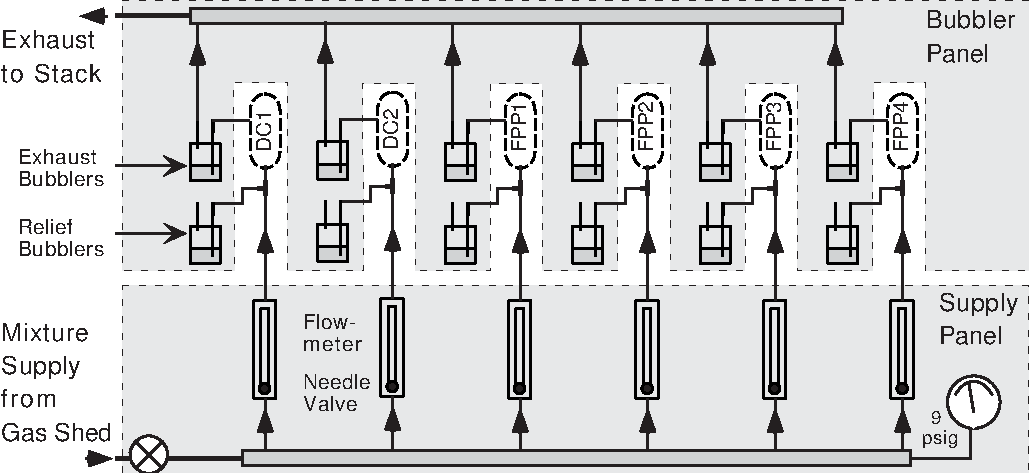
\includegraphics[width=\textwidth]{HMS_Gas_Circuit.pdf}
\caption{Flow and Valve Diagram for the HMS Shield House. An equivalent
installation will service two drift chambers in the SHMS Shield House.}
\label{fig:HMS_flow}
\end{center}
\end{figure}

The gas flow control electronics
and gas handling system are located in the gas shed just outside
of the Hall~C counting house.  See section~\ref{sec:chambergas} for details.

\paragraph{Electronics Operating Procedures}

The readout electronics associated with the HMS drift chambers are all
commercial products from LeCroy Research Systems, Nanometrics, CAEN
and Wiener.  There are 544 electronics channels per chamber for
a total of 1088 readout channels.  (588 per chamber, 1176 total
for the new chambers).

%FIXME BDS: do the HMS chambers still use both LRS and Nanometric cards?
These anodes are read out using LRS 2735DC
and Nanometrics N-277 preamplifier/discriminator cards mounted directly
on the chambers.  Each chamber has both types of cards, however each plane
(of six total planes per chamber) has only one type of card.  The
digitized signals are sent to VME CAEN 1190 TDCs inside of the detector hut
via twisted pair cable.  The low voltage (preamplifier) power supplies
(the Acopian supplies)
are in the 13 inch blue rack at the rear of the detector hut.  The
threshold voltage power supplies are on the frame under the Cherenkov
counter.  The remote
threshold power supplies are located in the electronics room of the counting
house.

\begin{center}
{\bf Procedure (in the detector hut)}
\end{center}

\begin{enumerate}
\item {Turn on low voltage power supplies (the Acopian Supplies).}
\item {Turn on threshold voltage power supply to appropriate setting.}
\item {Turn on the VME Crate power supply if it is not already on.}
\end{enumerate}

The threshold voltage
can be controlled locally in the detector hut or remotely in the
counting house. There is approximately a one volt drop in the threshold
voltage line in going from upstairs in the counting house to
downstairs in the detector hut.  Hence the supplies in the counting
house should be set to 5.5 volts. The local/remote switch is on the
controller in the
detector hut.  It should be switched to remote before exiting the hut.  The
LeCroy preamp/disc cards have LEDs (a green and a red light) which indicate
that the power is delivered properly to the chamber electronics.

\paragraph{High Voltage Operating Procedures}

Only formally authorized person may alter drift chamber high voltage.
There are four different voltages per chamber which must be turned on at the
proper time and monitored throughout the experiment.  {\bf MAKE SURE THAT
GAS IS FLOWING THROUGH THE CHAMBERS AND THAT THERE ARE
EDGE
CARDS MOUNTED
ON ALL READOUT CHANNELS BEFORE TURNING ON HIGH VOLTAGE.}
The high voltage
power supplies are the CAEN supplies located in relay rack CH03B17 in
the counting house electronics room.  The
voltages are set remotely using the GUI in the counting
house. See section \ref{sec:highvoltage} for information on
the high voltage controls.
The four different voltages are (nominally): triangle
wires (corner field wires) (-2500 V),
square wires (-2250 V), circle wires (-1800 V), and guard wires (-1500 V).
Note that each HMS drift chamber {\em plane} has its own triangle, circle,
and square voltage source, while there is only one guard wire voltage
source per {\em chamber}.
\begin{center}
{\bf Procedure (in the detector hut)}
\end{center}

\begin{enumerate}
\item {Make sure an amplifier/discrimator card or a grounding plate is on each instrumented
connector on the chamber.}
\item {Make sure that there is gas flow, particularly Ar gas.}
\item {Make sure high voltage cables are properly connected to
chamber.}
\item {Turn on high voltage, using the EPICS GUI in the counting house,
to proper settings.}
\end{enumerate}

%The CAEN power supplies, when operated remotely, are controlled by the
%EPICS control system.  To operate, log on to vxworks, get the high
%voltage monitors (use the rightmost mouse button to bring up the menu)
%and choose the chamber voltage group.  Each high voltage channel is
%independently controlled.

In general all of the voltages and gas flow should be left on, even when
no data is being collected.  The gas supply should be checked periodically,
approximately once every shift.  The gas bottles' supply is depleted
after about 2 weeks at the nominal (400 cc/min) flow rate.
In the case of a HV trip, try cycling the CAEN power supplies.  If this fails, call
one of the responsible persons listed in the Responsible Personnel Section
of the \htmladdnormallinkfoot{ESAD}{http://www.jlab.org/Hall-C/document}.




\subsection{Scintillator Hodoscopes}

The purpose of the scintillator hodoscopes is to provide a clean
trigger as well as particle identification by time of flight (TOF). These
detectors consist of two pairs of spatially separated scintillator
layers: a pair comprised of S1X and S1Y, and approximately 2 meters away a pair
comprised of S2X and S2Y. General characteristics of the BC404 scintillator
material are as follows:

\begin{itemize}
\item{Polyvinyltoluene (PVT) is the base material. }
\item{Light output is 68\% that of Anthracene. }
\item{Wavelength of maximum emission is 408 nm.}
\item{Decay constant of the main fluorescence component is 1.8 ns.}
\item{Bulk attenuation length is 160 cm.}
\end{itemize}

	The specific dimensions for the scintillator elements in the HMS
are found in Table~\ref{tab:tof_scintillators}.
\begin{table}
\caption{Dimensions (at 70~F.) of the scintillators for the HMS TOF system.
\label{tab:tof_scintillators}}
\begin{center}
  \begin{tabular}{ccccc}
	&Thickness	&Width		&Length		&Number	\\
	&		&		&		&	\\
\hline
X(HMS)	&	1cm	&	8.0cm	&	75.5cm	&32 units\\
Y(HMS)	&	1cm	&	8.0cm	&	120.5cm	&20 units\\
  \end{tabular}
\end{center}
\end{table}
Each scintillator is read out by two Philips XP2282B photomultiplier
tubes (PMT's). These PMT's are 8-stage tubes with nominal operation at
2500 volts. The bases have two anode outputs, one of which is terminated with a
short clip line and 40 Ohms.  Because of pmt to pmt variations in gain and the
5\% precision zener diodes in the bases, the spread in gains can be a factor of
2-3. Individual high voltages must therefore be adjusted to balance the gains.
The gains have been carefully matched with a source, and HV save files exist,
so the gains will not normally need to be readjusted. If gain adjustment is
necessary, inform one of the hodoscope contact persons as soon as possible.
Mysterious gain shifts are probably due to transient problems like bad solder
contacts or broken glue joints. They require repair. A rough rule of thumb is
that an increase of 50 volts will increase the gain by 30\%.

With our base, the HV channel will trip on overcurrent (3 mA) at 2900 V
(this base is essentially divider C in the Philips catalog). If a channel needs
more than 2800 volts, and the base and glue joints are okay, then our policy
is to replace the pmt. We have several spare modules in the counting room.
In desperation, ``spares" can be taken from the edges of the acceptance. In the
HMS, S1X16 or S2X16 contain little or no useful data, and similarly for S1Y01
or S1Y10.

	The light guide material is UVT lucite.  Wrapping material for the SOS scintillator elements was one layer of
aluminized mylar (aluminum side facing inward), followed by two layers of
tedlar for light tightness. The HMS elements were wrapped in aluminum foil,
followed by one layer of tedlar.

The HMS elements are supported at the lightguides. In case of repair use BC-600
glue. Each element has a 1 mm plastic fiber glued into the light guide. These
fibers are also very delicate and care must be taken when moving a scintillator
element to avoid snagging and breaking the fibers.

{\bf What to check}: Before starting to operate the detectors, one has to
check the trip setting (current limit) of the HV power supply for each channel
and the set HV value of each channel. During operation, the current of each
channel and its HV should be periodically checked. The HV should be on for at
least half an hour before taking data. During runs one should check the
histogram of the plane hit distribution. This should be rather flat reflecting
the normal trigger requirement of 3 out of 4 planes. Also the element hit
distributions for the individual planes should be checked regularly. These
distributions are defined for both ends of the elements using both ADC and TDC
information.

{\bf Nomenclature}:
The coordinate system (right handed, following TRANSPORT
convention) is defined as z downstream, x pointing down, and when looking
downstream, y to the left. In this convention the X-tubes at positive Y are
called X+ and the Y tubes at the bottom (pos x ) are called Y+. Numbering of
the elements is done as one would read a book in English: left to right in the
case of the Y and top to bottom in X.

	There are one ADC and one high resolution (25 ps/channel) TDC per PMT.
For the SOS, S1X and S1Y and S2Y each have 18 channels, while S2X has 32 making
it 86 channels in total. Each ``X''plane in the HMS has 32 and each
``Y'' has 20, making it 104 channels in total.

	The signals are carried on an RG-8 size cable which is a Belden 213
equivalent. The nominal specifications are 50 Ohm impedance and the signal
velocity is 0.82c . The signals are passively split in the counting house with
one going to the ADC and one going to leading edge discriminators. The
performance is typically 150 psec mean time resolution (sigma) per
element.

\subsection{Gas Cherenkov Detector}

A charged particle travelling faster
than the speed of light in the medium will create an electromagnetic
disturbance in the medium. The radiation emitted by this process is
called Cherenkov radiation after its discoverer.

Cherenkov radiation is conically distributed about the trajectory of the
particle, with an angle given by
$$
	\cos{\theta} = \frac{1}{\beta n}
$$
where the index of refraction $n = c/u$ and $\beta = v/c$, with $c$
the speed of light in vacuum, $u$ the speed of light in the medium,
and $v$ the speed of the particle.

The index of refraction allows one to control the threshold particle velocity
$v_{T}=u=c/n$ below which there is no Cherenkov light produced, and above which there
is Cherenkov light produced.  For a gas, the quantity $n-1$ is proportional to the pressure,
so adjusting the pressure of the gas allows one to select the
threshold velocity. Adjusting the threshold velocity actually allows one to select particles of
different mass.  Given the same momentum, two particles of different mass
will have different velocity.  Therefore, a Cherenkov detector can be tuned,
for instance, to distinguish electrons from pions.

	The HMS Cherenkov detector consists of a large cylindrical
tank, $\phi_{in} = 59"$, $L = 60"$, containing two mirrors which focus
light onto two 5 inch Burle 8854 multiplier photo  tubes (PMT's). The tank
has been installed with 0.04 inch thick 2024-T3 Aluminum windows
covering the circular ends of the cylindrical tank. These
windows were hydrostatically formed (and hence tested) at a pressure
of 28 PSI. The tank itself was helium leak checked and is leak free
on a scale of 10$^{-8}$ Atm-cm$^3$/s. In addition, the tank was hydrostatically
tested at a pressure of 35 PSI. Detailed information on this testing
program can be found in \cite {bi:tank}, \cite {bi:wind}.

The tank is mounted on the detector rails using a three point
alignment scheme. The rails are easily capable of supporting the
weight of the tank without deformation.
The gas handling system for the tank
is designed to enable the tank to be filled with
pure gas, CO2 or N$_2$, at the desired operating
pressure which is, $\approx$ 1 Atm (11.5 PSI) for the near future.

The system consists of the fill gas bottle and primary
pressure regulator which are in a bottle rack that's welded to
the bottom of the HMS detector hut on the small angle side at a height
of about six inches from the hall floor. The primary regulator is
a Matheson model 2596 with a maximum outlet pressure of 400 PSI.
During fills this regulator should be set to 150 PSI.
The outlet of this pressure regulator is connected to the
main gas control panel which is mounted on the first floor balcony
of the detector hut behind the dipole control racks. All connecting
tubes in the system are 0.25 inch diameter stainless steel tubing with
the exception of the nitrogen purge line which is thick wall tygon.
At the entrance to the gas panel there is a 0-300 PSI gauge so that
the pressure in the inlet line can be viewed by the operator.
The line is then relieved by a Circle Seal relief valve set at 200 PSI.
After this, the gas passes through a second regulator (Matheson 3420)
which has an
outlet pressure range of 0-60 PSI. This regulator can be set at
up to 40 PSI for high flow during the early stages of fills
(the line is relieved further downstream by a second
Circle Seal relief valve set at 45 PSI) and then reduced as
the desired operating pressure is approached. Following the second regulator
and its relief valve the gas passes through oil and oxygen filters.
A 120 Volt AC solenoid valve (ASCO) switched with a solid state
relay is used to isolate the gas flow from the tank. The state of
the relay and hence the valve is indicated by a LED on the panel.
The gas line is routed through an opening in the floor of the detector hut
to the tank inlet. A gauge on the panel allows the operator to view
the pressure in the inlet line (the same as the tank pressure
when the subsequent manual valve is open, see following).
At the inlet there is a pair of manual valves (NUPRO)
which allow the fill line to be purged.
During operation the valve which vents the
line to atmosphere is closed and the valve to the tank inlet is open.
The tank is relieved by a 1 inch diameter, 1 PSI pop off (NUPRO) which was
sized to take the
maximum flow of the second regulator even if that regulator has failed
wide open. There is a pressure gauge on the tank so that its condition
can be determined by workers in the shield house. In addition,
there is a Omega pressure transducer (PX-305-05A) and a temperature
transducer attached to the tank. These are read out and powered by
units (Omega) which are located below the gas panel.  Outputs of these
are currently viewed with a video camera attached
to a monitor in the counting house.

Before filling, the tank is first cleaned by executing several pump
and purge cycles. The pump that is used to evacuate the tank is located on a
platform welded to the small angle side of the shield house balcony
which can be accessed from the small angle side of the HMS carriage.
Eventually, it will be possible to switch the power for this pump
from the gas control panel with a relay but currently it
is necessary to turn the pump on and off with a switch located on the pump.
The low pressure side of this pump is equipped with a liquid nitrogen
cold trap to prevent any contamination of the tank (or mirrors !)
with pump oil. This trap will remain filled for approximately
12 hours and should always be checked before use. There is currently
a manual valve located at the Cherenkov tank that isolates the tank from
the pump.  This valve will later be replaced by a pneumatically actuated
solenoid valve that will be controlled from the gas panel.
There is a manual valve on the tank which is equipped with a hose
barb through which clean nitrogen purge gas can be admitted to the tank.
The nitrogen gas comes from a spigot on the HMS cryogenic handling system
located along the upper catwalk of the HMS. The nitrogen system
delivers gas at a line pressure of $\approx$ 40 PSI (this pressure can
be read on a gauge at the pivot end of the catwalk). The flow
rate is readable from a flow meter attached to the spigot. A flow of
about 150 - 200 cfm is reasonable. The tank should not be filled to
more than -5 in Hg during purge cycles.

The tank contains two 5 inch PMT's which use {\bf positive} HV.
(Note: only this detector and the Aerogel counter use positive HV, all the other PMT bases in the HMS are designed for use with
negative HV.) They operate
at between 2000 and 2700 Volts. The Anode is at HV and its signal is
viewed through a decoupling capacitor in the base. The HV is supplied
by one pod of the same {\em CAEN} power supply used for the drift chambers.

The mirrors in the tank may require adjustment for optimal focusing
on the PMT faces. The ports which hold the PMT's are sized big enough to allow
a person inside the tank to make these adjustments. The tank is a confined
space and hence this activity represents an ODH hazard. Stickers indicating
this have been placed on the PMT ports. Before an entry into the tank the
atmosphere in the interior must be surveyed by a member of the physics
division EH$\&$S staff.
This adjustment should only
be done by personnel who understand the fiducial markings of the PMT
mounting system. The interior of the tank has foot braces and hand holds welded
to allow this work at the angle of the detector rails.

\paragraph{Operation Procedures}

\begin{figure}
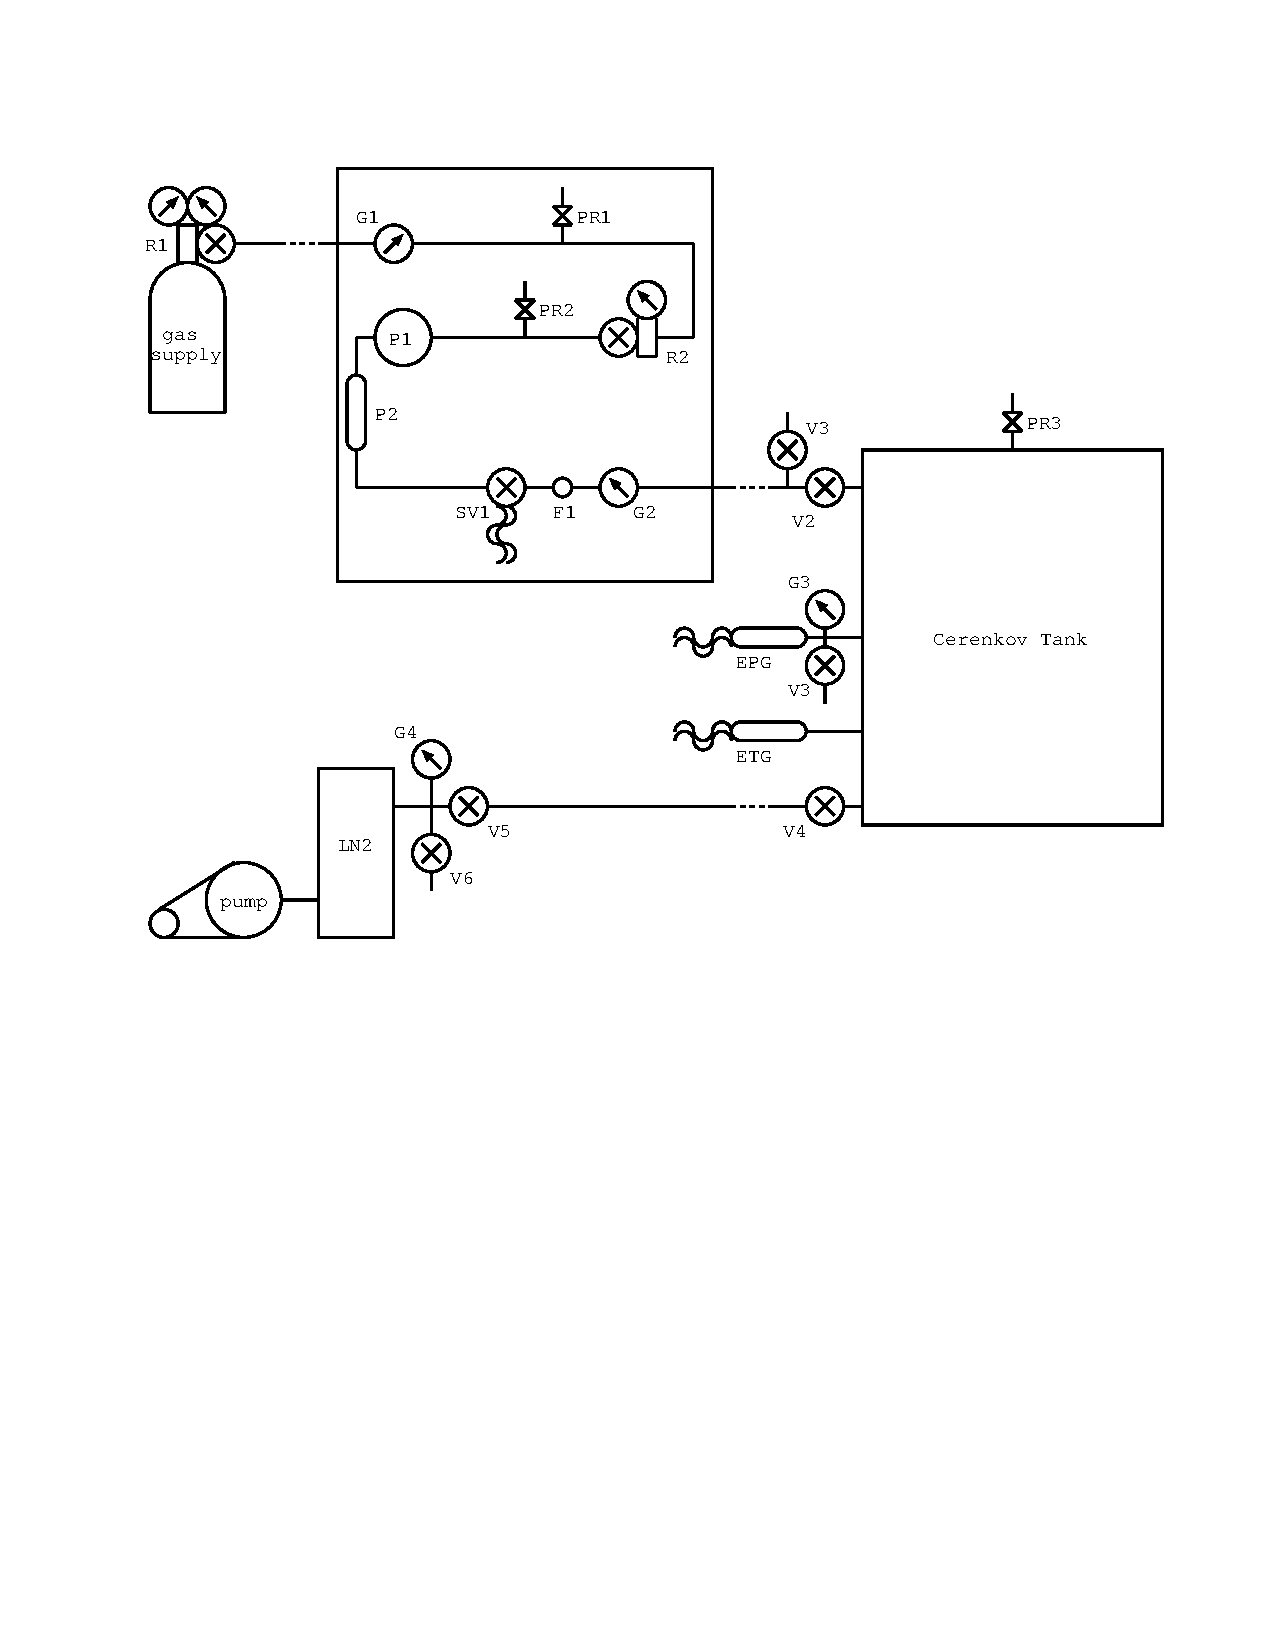
\includegraphics[height=4in,trim=20 300 20 40,clip]{HMSgasC.pdf}
\caption{The Gas Handling System for the HMS Cherenkov Detector. \label{fig:gas}}
\end{figure}

The HMS Cherenkov Detector operates either as an $e/\pi$ or $\pi/p$
discriminator. Each mode has a unique set of procedures to prepare the tank
for operation. The nomenclature used in the description of these operation
procedures refers to Figure~\ref{fig:gas}, showing the gas handling system. Components
shown
inside the dashed box of Figure~\ref{fig:gas}, are all located on the Gas Control Panel.

\paragraph{$e/\pi$ Procedures}
For both $e/\pi$ and $p/\pi$ separation, the procedure
has been to run with 0.4 to
0.9 (?) atmospheres of C4F10.  This is just a small modifiction to the
current p/pi procedures write-up described in the next section,
with the HMS running sub-atmospheric instead of supra-atmospheric.

$e/\pi$ running can also be accomplished using a nitrogen fill.
This mode of operation requires the tank to be filled with approximately
13.5~psia of $\rm{N_2}$.  The boiloff from the spectrometer magnets is a
perfect source of clean, dry Nitrogen, and is normally used to fill the
Cherenkov tank.

Because the operating pressure is slightly subatmospheric, a pump and fill
procedure is employed.  First make sure that:
\begin{itemize}
\item The 40~mil windows are installed and oriented such that they curve
towards the interior of the tank.
\item Valves {\bf V1-V6} are closed.
\item The LN2 trap is filled.
\item There is enough oil in the pump.
\end{itemize}
The tank is now ready to be evacuated.
\begin{itemize}
\item Turn on the pump.
\item Slowly open {\bf V5}.  This evacuates the pump line.
\item Very slowly open {\bf V4}.  Since this valve connects the pump line to
the detector volume, the pump will work very hard.  Meter this valve
so that the pump is never under extreme stress.  It will take approximately
20~minutes to pump down the tank.
\end{itemize}
The tank can now be filled.
\begin{itemize}
\item Locate the boiloff manifold on the walkway on the top level of the
spectrometer, at the gap between Q3 and the dipole.
\item Turn the valve on this manifold open slightly so that the flow meter
barely registers a flow.
\item Connect the remaining end of the Tygon tubing to the vent of valve
{\bf V3} with a hose clamp.
\item Open valve {\bf V3}.
\item Increase the flow on the flow meter.  Do not exceed 100~cfpm.
\item When {\bf G3} or {\bf EPG} reach the operating pressure, close
the manifold valve.
\item Close {\bf V3}.
\end{itemize}
The fill should take approximately 30 minutes.  The detector should NEVER
be left unattended during a fill.  Frequently check the pressure in the tank
and be aware when the pressure nears one atmosphere.  DO NOT let the pressure
exceed one atmosphere under any circumstances; doing so risks damage to all of
the equipment and personnel in the detector hut.  This pump/fill procedure is usually
repeated at least once to insure the
purity of the gas.

\paragraph{$\bf{\pi}/p$ Procedures}
This mode of operation typically requires the tank to be filled with Freon-12
at pressures varying from 2 to 3~atm.  Because these operating pressures are
greater than 1~atm, the detector must be filled by dilution.  Contamination
from air, however, is not a major problem as the optical absorption properties
of air are actually more favorable than those of Freon-12 itself; the only
difficulty is the increase in pressure needed for a mixture of air and Freon
to achieve the same pion momentum threshold as for a pure sample of Freon.

First prepare the gas handling system:
\begin{itemize}
\item Make sure that the 60~mil windows are installed and oriented such that
they bulge outwards from interior of the tank.
\item Close the valves {\bf V2-V4}, and the valve on regulator {\bf R1}.
{\bf V1}, {\bf SV1}, and the valve on regulator {\bf R2} should be
open.
\item Open the valve on the gas supply bottle.
\item Adjust {\bf R1} to approximately 60 psig.
\item Open the valve on {\bf R1}.
\item Check to make sure gauge {\bf G1} agrees with the pressure setting
on {\bf R1}.
\item Adjust {\bf R2} so that a small flow is detected out the vent of
{\bf V1}.
\item Close {\bf V1}.
\item Adjust {\bf R2} to regulate at the required operating pressure.
\end{itemize}
The tank is now ready for the dilution process.  These steps should be
repeated as few times as possible to minimize the quantity of Freon-12 emitted
to the atmosphere.
\begin{itemize}
\item Record the tank pressure.
\item Open valve {\bf V2}.
\item Monitor the gas pressure until it reaches the required operating pressure.
NEVER let the pressure in the detector exceed 3~atmospheres.
\item Record the final pressure.
\item Open {\bf V3} to vent the tank.
\end{itemize}
From the recorded pressure readings, the threshold momentum of the mixture
of air and Freon-12 can be calculated (assuming the volume of the tank is
fixed).



\subsection{Lead Glass Shower Calorimeter}

The HMS lead glass shower
calorimeter~\cite{Mkrtchyan201385}
consists of four stacks of
TF1 leaded glass (similar to SF1). Each stack contains thirteen
blocks for a total of 52 blocks. The blocks are 10 cm by 10 cm by 70
cm.  The first two layers are readout with PMTs at both ends and the
last two layers with a PMT at one end.

High energy particles
emit Cherenkov radiation when passing through the glass and a signal
is collected that is proportional to the sum of the path lengths
travelled by all the
particles which are above the threshold for Cherenkov emission. High energy
electrons will produce a large signal as they have a large bremsstralung
cross section and the photons which are produced in the bremsstralung
process have a large cross section to produce electron positron pairs
(all of which will be above the Cherenkov threshold). This process
of bremsstralung followed by pair production is called an electromagnetic
shower.

The histograms associated with the calorimeter should be inspected
regularly to assure that it is functioning properly.

\section{Aerogel Detector}
The HMS Aerogel detector\cite{Asaturyan2005364} is located between the
second wire chamber and the first plane of the hodoscopes.  It
provides improved $\pi/K/p$ particle ID for momenta above
$3~\textrm{GeV}/c$.  The detector is mounted on a sliding rail system
so that it may easily be placed into or removed from the path of
particles in the detector hut depending on the needs of a given
experiment.

The Aerogel detector, which has an area of $120\times
70~\textrm{cm}^2$ consists of a 9 cm thickness of Aerogel followed by a
diffusion box for a total thickness of 25 cm. The diffusion box is
line with Millipore paper ``Membrane GSWP-0010'' which has a
reflectivity of $\sim 96\%$ \cite{millipore}.   The ``long'' sides the diffusion
box each have 8 Photonis XP4572 PMTs.  These bases for these tubes are
powered with positive HV.
(Note: only this detector and the gas Cherenkov detector
use positive HV, all the other PMT bases in the HMS are designed for
use with negative HV.)

Two Aerogel indices of refraction, $n=1.015$ and $n=1.030$, are
available for use with the detector.  The Aerogel is in radiator
trays which may be swapped (by experts) to change the refraction
indexed installed in the detector.


\begin{table}
\caption{Momentum threshold above which pions, kaons and protons will
produce Cherenkov light in Aerogel's with various indices of refraction.
\label{tab:hms_aerogel}}
\begin{center}
\begin{tabular}{cccc}
  n& $\pi_{\textrm{thr}}(\textrm{GeV}/c)$ & $K_{\textrm{
  thr}}(\textrm{GeV}/c)$ & $p_{\textrm{thr}}(\textrm{GeV}/c)$\\
  1.030 & 0.57 & 2.00 & 3.80 \\
  1.015 & 0.81 & 2.84 & 5.40 \\
\end{tabular}
\end{center}
\end{table}

}%\infolevone

\infolevone{
\section{The SHMS Detector Package and Shield House }

The Super High Mometum Spectrometer contains two separate shielded
rooms.  The first room, referred to as the electronics hut, contains
electronics associated with the trigger and data acquisition system as
well as magnet power supply controls.
(Figure~\ref{fig:shmshuts})
This room is entered through a concrete
door on the second stairway landing of the spectrometer structure.
The second shielded room, known as the detector hut, is accessed by
passing through the electronics hut.  These rooms are separated a
sliding concrete door.  Both doors must be closed during beam
operations.  The electronics and detector huts have removable ceiling
and wall sections in case detectors or electronics racks need to be
removed or installed.  Jerry Nines, the Hall~C work coordinator,  
must be contacted if the hut walls or ceilings need to be removed.
\begin{figure}
\begin{center}
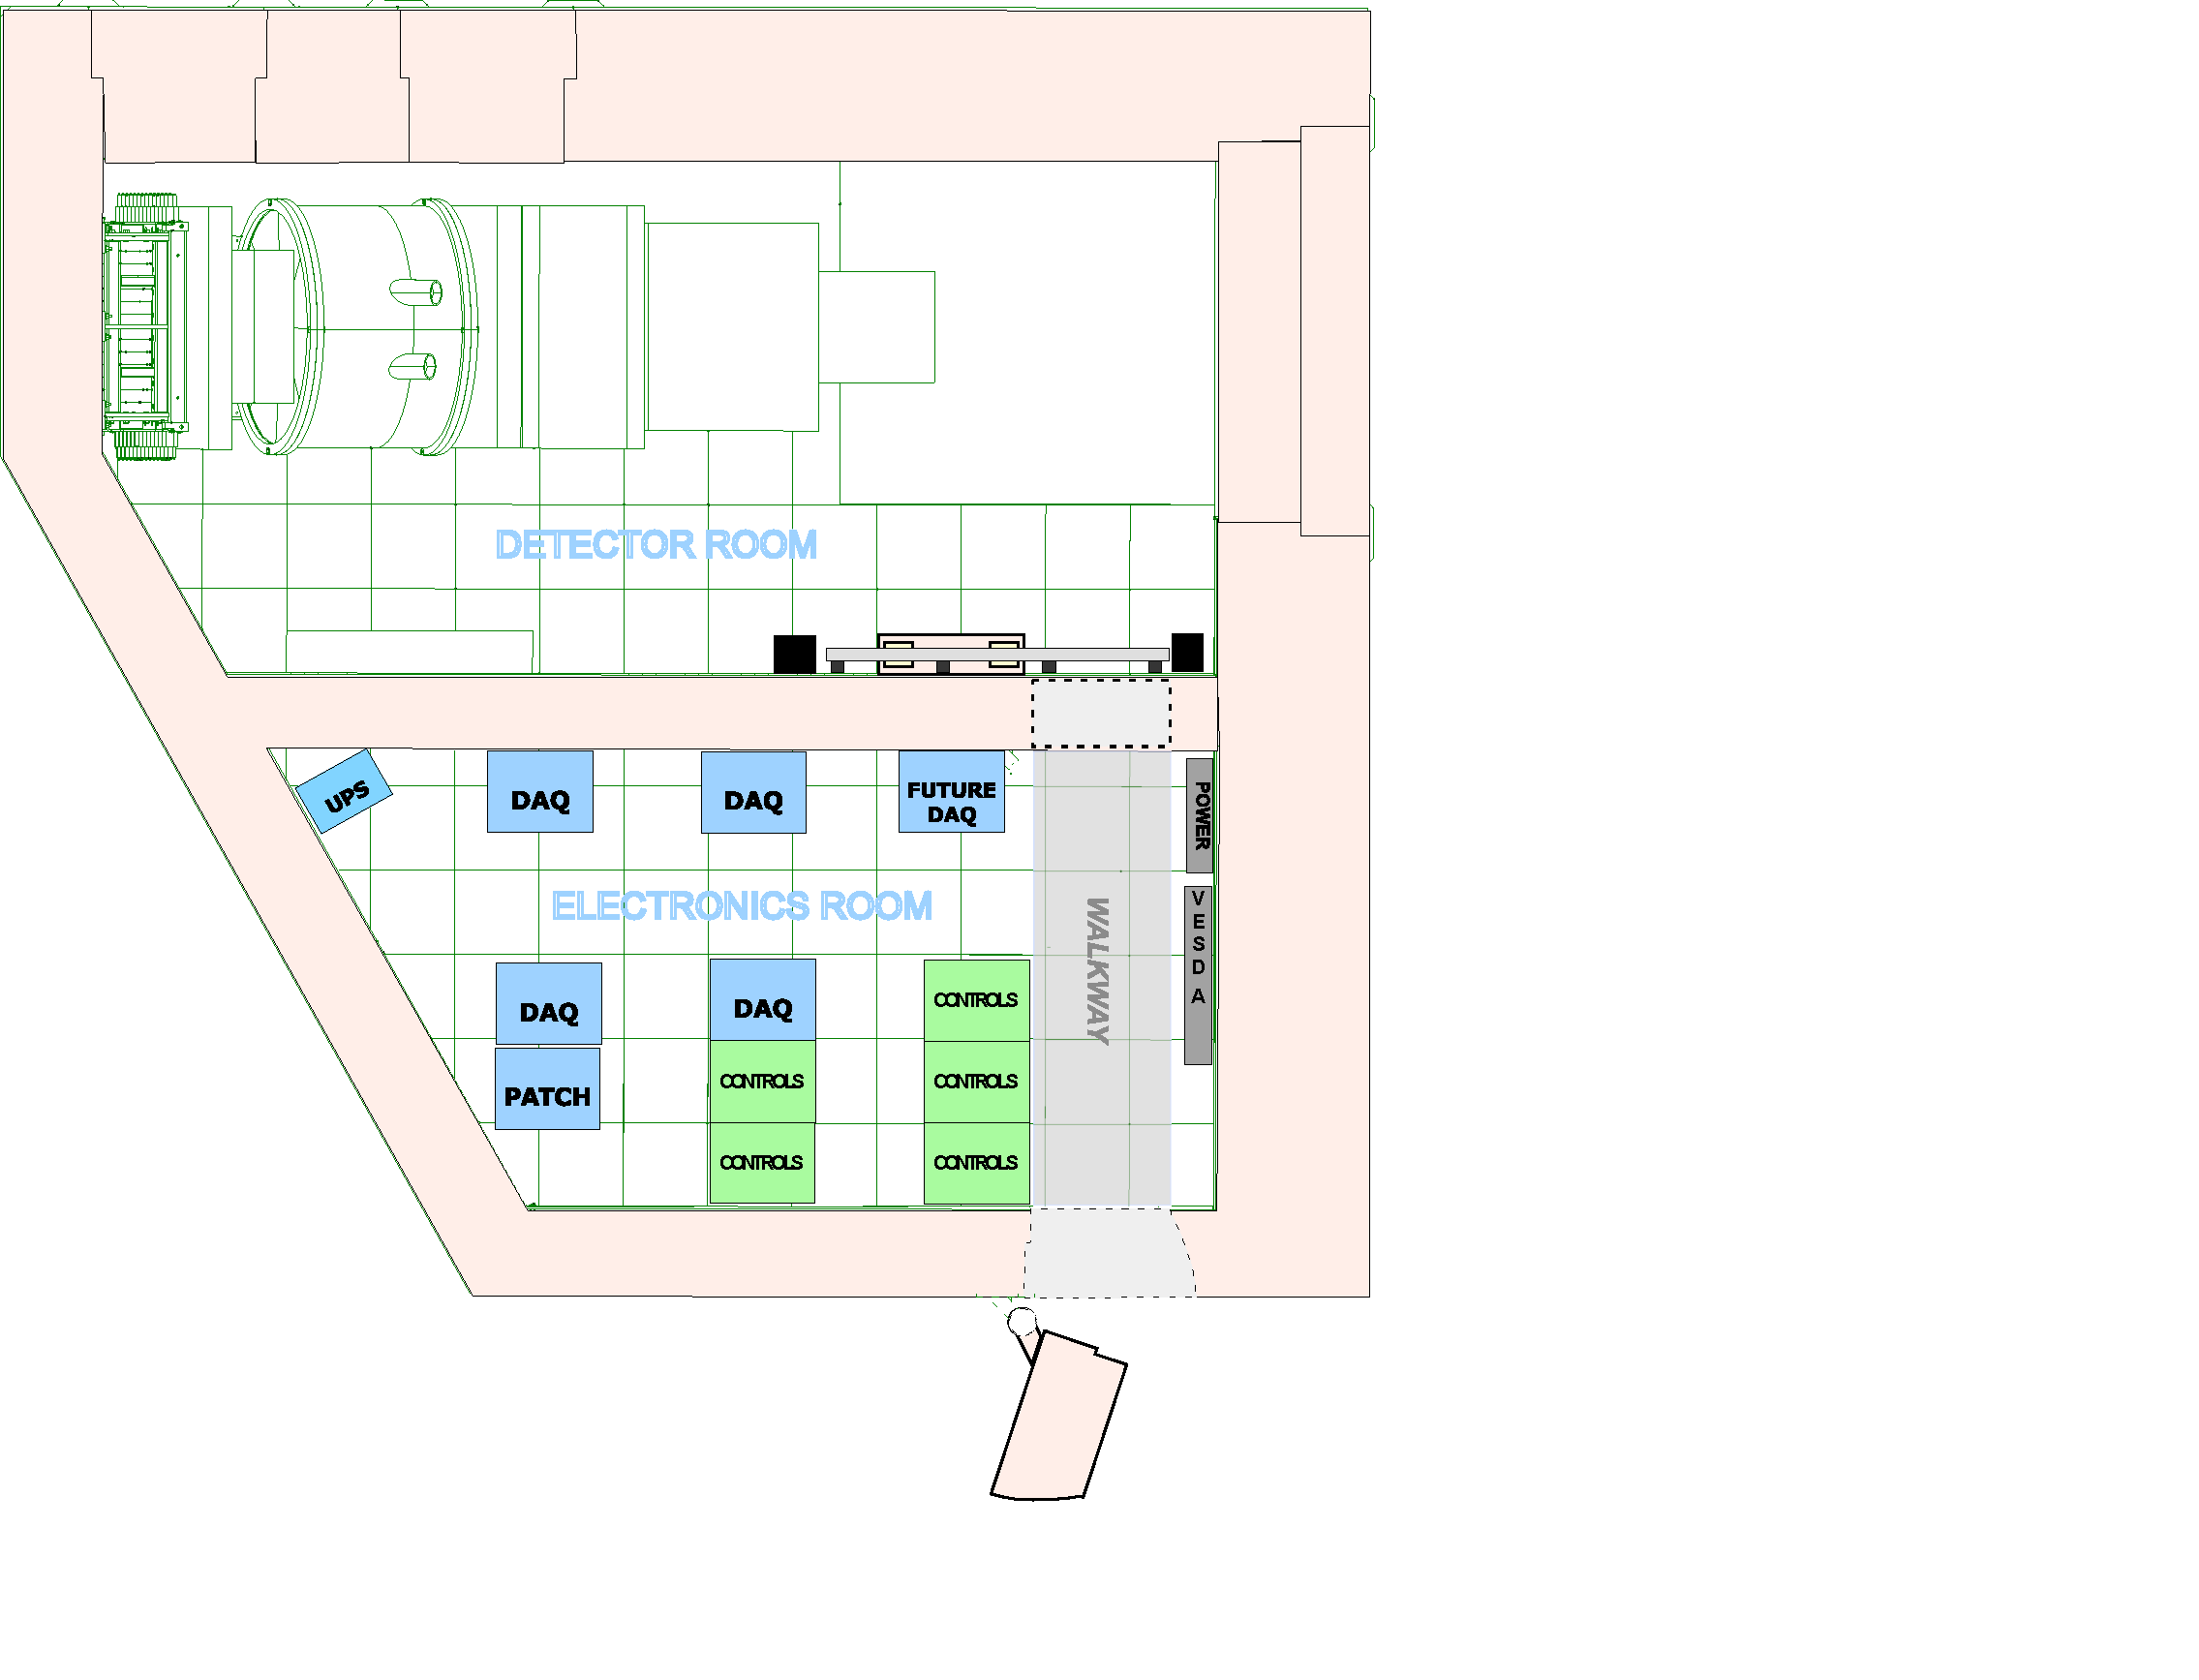
\includegraphics[width=5in]{ShieldHutRacks_hcfAsBuilt.pdf}
\caption{\label{fig:shmshuts}SHMS Detector and Electronics huts,
  accessible from the second level of the SHMS structure.  The
  detectors are accessible by passing through the electronics room.}
\end{center}
\end{figure}

\begin{figure}
\begin{center}
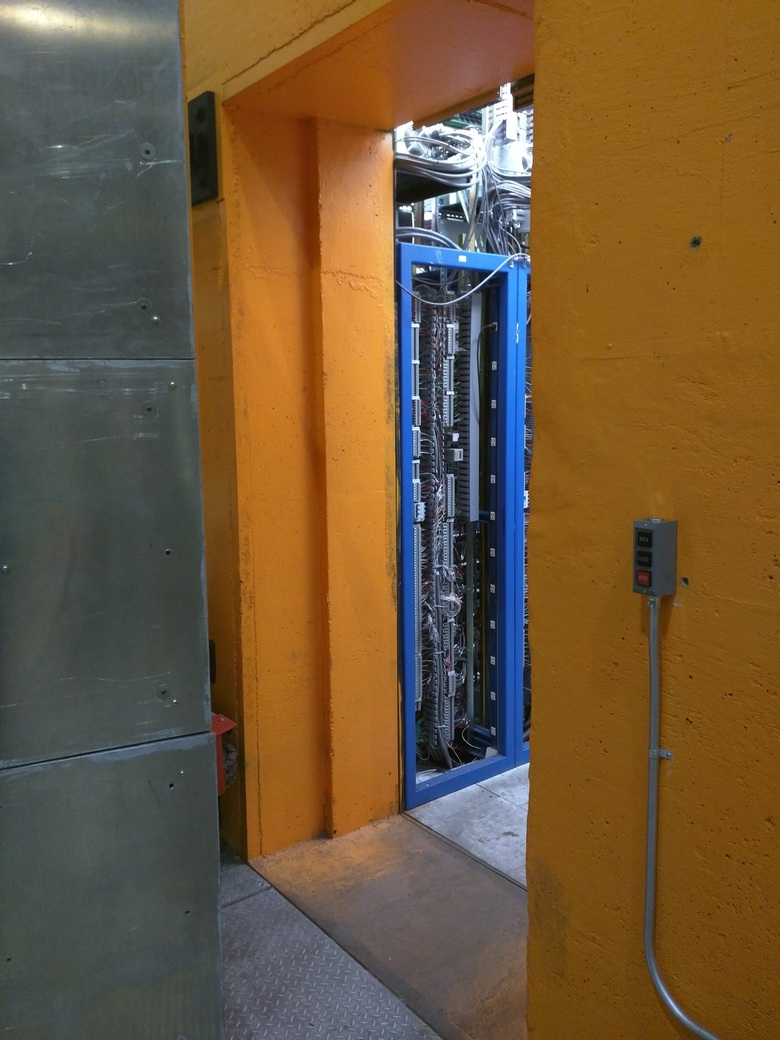
\includegraphics[width=4in]{shmsdoor.jpg}
\caption{\label{fig:shmsdoorcontrol}SHMS hut outside door control buttons.}
\end{center}
\end{figure}

\subsection{SHMS Electronics and Detector Shield Hut Doors}
\label{sec:shmsdoors}
The SHMS electronics shield hut is accessed through concrete door held
closed by a magnetic lock.  To open this door, press and hold the
button marked OPEN.  (Figure~\ref{fig:shmsdoorcontrol})  This will
deenergize the magnetic lock and rotate
the door.  When the door is open sufficient for access, release the
button.  To close the door, make sure the door is clear of
obstructions and hold the CLOSE button until the door closes and the
magnetic lock activates.  A duplicate set of controls is located on
the inside of this door.  When the door motor is energized, audible and visual
alarms will be activated.

The detector shield hut is accessed by passing through the electronics
hut and passing through a second door.  This door is a sliding door
(``barn door'') and is operated by the lower set of buttons to the
right of that door (Figure~\ref{fig:barndoorcontrol}).  This door is activated
in the same manner as the outer electronics hut door: The door slides open
while the OPEN button is depressed, slides closed when the CLOSE button
is depressed and movement stops when the button is released.  Audible and
visual alarms are also installed for the sliding door.
If the spectrometer
vaccum window has a shutter installed, then this door may only be
opened if that shutter is closed.  This shutter is described in the
next section.

An emergency bypass is available allowing override of the shutter
interlock on the door.  Hearing protection must be worn if detector
hut is accessed while the shutter is open and the spectrometer is
under vacuum.

\begin{figure}
\begin{center}
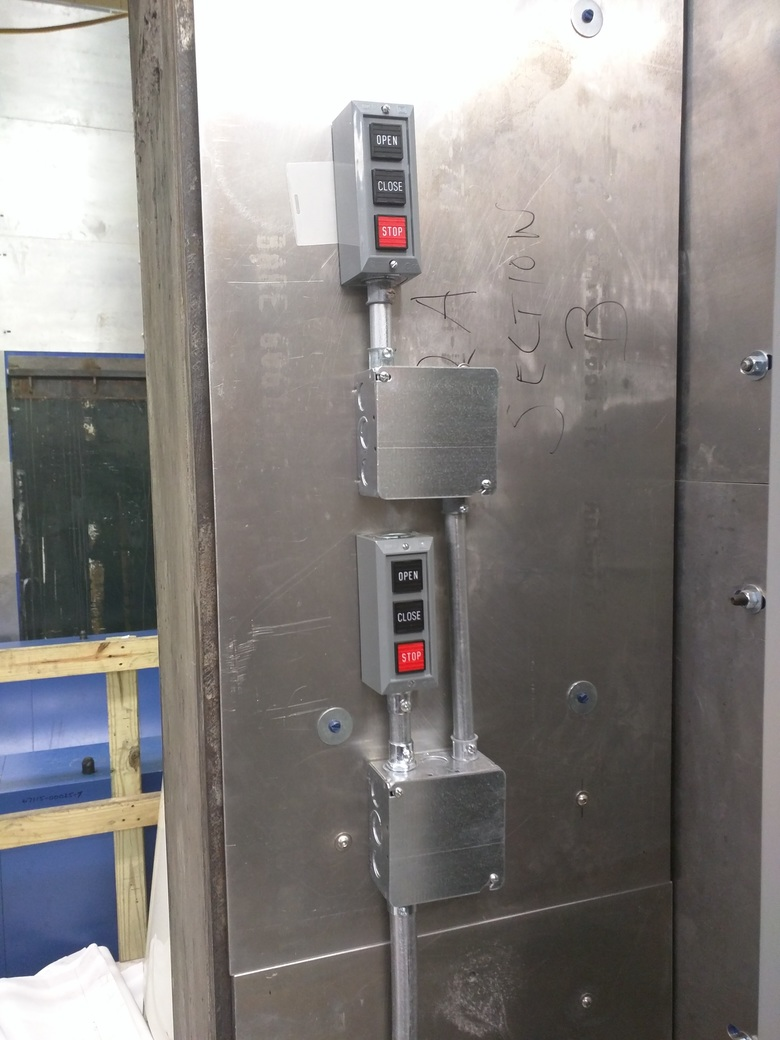
\includegraphics[width=3in]{barndoor-outside.jpg}
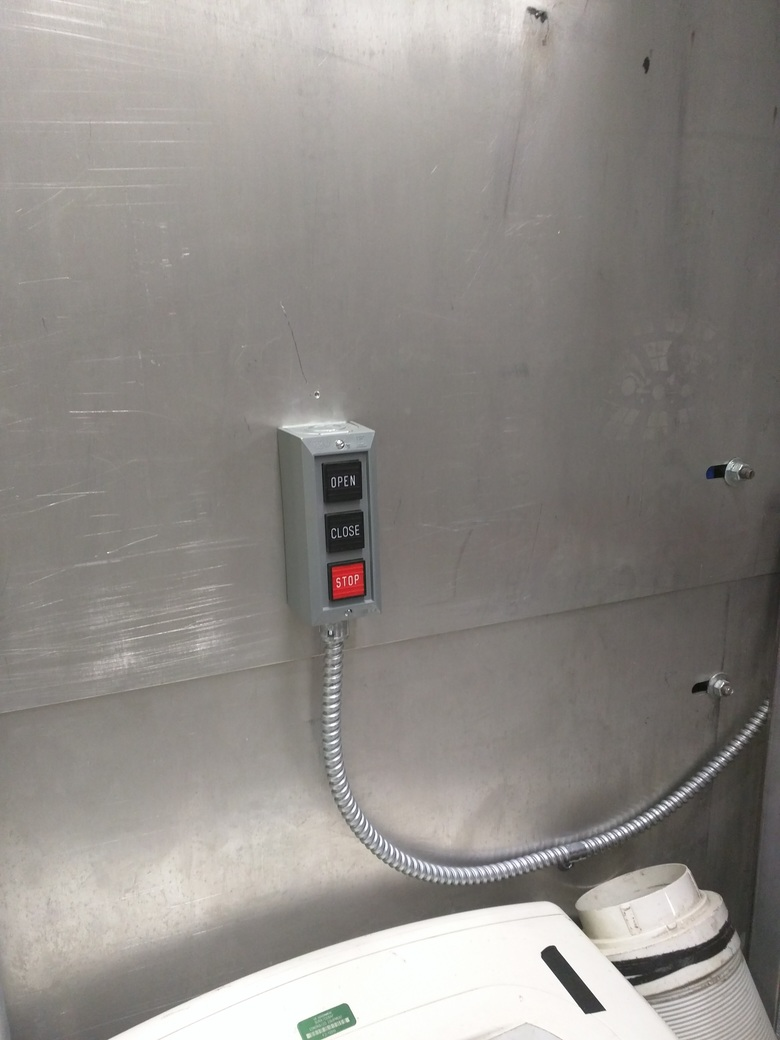
\includegraphics[width=3in]{barndoor-inside.jpg}
\caption{\label{fig:barndoorcontrol}SHMS barn door controls.  The left
  picture shows the controls located in electronics hut.  The bottom
  buttons control the barn door. The top buttons control the SHMS
  vacuum extension shutter.  Below the shutter controls are lights
  indicating if the shutter is opened or closed.  The right picture
  shows the barn door controls located inside the detector hut.}
\end{center}
\end{figure}

\subsection{SHMS Vacuum Window Shutter}
\label{sec:shmsshutter}
As described in section~\ref{sec:shmswindows}, there is a large thin
vacuum window at the end of the vacuum pipe in the SHMS detector hut.
Because of
the considerable stored energy in such a large vacuum volume, it is
necessary to protect the window from accidental puncture by
tools and equipment.
If
the Noble Gas Cherenkov detector is installed, protection is provided
by that detector.
If the Noble Gas Cherenkov is not installed, a vacuum
extension pipe, with a window further into the detector hut will be
used.  In this case, the window will be covered by a shutter to
protect the window from being punctured by tools.
This shutter must be in place whenever the spectrometer is under vacuum and
the ``barn door'' is open.  The shutter is operated by using the top
set of buttons shown in Fig.~\ref{fig:barndoorcontrol}.  To open or close
the shutter, momentarily press the OPEN or CLOSE button.  The shutter will move
until it reaches the open or closed state. (Unlike the door controls,
the button does not need to be held down.)  Indicator
lights near the shutter and door controls show whether the shutter is open or closed.




}%\infolevone

}
\begin{safetyen}{0}{0}
\infolevone{\section{Safety Information}}
\label{sec:spectrometer-safety}

\subsection{Hazards}

The spectrometers have associated vacuum, electrical, cryogenic and
magnet systems all of which can be extremely dangerous due to the size
and stored energy in the systems.
Parts of the spectrometers are at elevated levels which would present fall
hazards if the installed safety equipment were not present.
Hazards of rotating the
spectrometers as well as the particle detectors that get placed inside
the detector hut of the spectrometer are covered in detail in
following sections.

Signage and alerts are placed to remind workers of some of the potential hazards
in Hall C, but each individual is ultimately responsible for his or her own
safety. Always read and respect warning signs, and never attempt to
circumvent barriers or other equipment
that has been installed for your protection. If you discover what appears to be a
new or unidentified hazard, protect your coworkers by warning them
and alert the Hall-C management and Safety Warden.

\subsection{Mitigations}

Both of the spectrometers have elevated work platforms that are secured by
gates and handrails. Never attempt to bypass these protections. During experiment
running periods, in order to allow spectrometer rotation, it may be necessary to
remove the handrails around the target platform. In this condition access to the
target platform is restricted to trained individuals who have been specifically
authorized to work near there. Fall-protection equipment is required.

The vacuum systems associated with the spectrometers are essentially
pressure vessels and care should be exercised so as not to damage or puncture the
vacuum windows.   The large vacuum windows inside the two shield houses are protected
by shutters which must be lowered into place before the access door to the
detector rooms will open. (When the Noble-Gas Cherenkov (NGC) is installed in the SHMS,
the NGC itself protects the vacuum window and the shutter is not present.)
During hall maintenance, covers are placed over the spectrometer
vacuum windows near the pivot to help prevent anything from accidentally hitting
a window. Hearing protection may be required when you work near a vulnerable
vacuum window. As conditions may change, please take note of currently posted
warning signs and instructions.

The magnets themselves are installed inside cryostats.  These vessels
are exposed to high pressures and are therefore equipped with safety
relief valves and burst discs.

The cryogenic system operates at an elevated pressure and at temperatures
about 4~Kelvin (helium system) and about 90~Kelvin (nitrogen system).  One must
guard against cold burns and take the normal precautions with pressure
vessels when operating or working near this system.  Manipulation of any cryogenic
system component such as a U-Tube or manual valve may only be performed by
a trained cryogenic-system expert.

When they are powered, the magnets have a great deal of stored energy as they are large
inductors.
\infolevone{(See Table~\ref{tab:magnet_parameters}.)}
Always make sure people are clear of
the magnets and their dump resistors.

\subsection{Responsible Personnel}

In the event that problems arise during
operation of the spectrometers, qualified personnel should be notified
(see Table \ref{tab:spec:personnel_technical}).
This includes any prolonged or serious problem with the source of magnet
cryogens (the ESR).
\infolevone{(See also ``Checking Cryogenics'' in Section \ref{ssec:operatemagnets}, below.)}
On weekends and after hours there will be a
designated individual on call for magnet services.  Any member of the
Hall C technical staff is qualified to deal with unusual magnet
situations but in the event of serious problems the person on
call should be contacted.

\begin{namestab}{tab:spec:personnel_technical}{Spectrometers: authorized personnel}{%
      List of spectrometer responsible personnel where ``W.B.'' stands for the white board
      in the counting house.}
   \TechonCall{\em Contact}
   \SteveLassiter{}
%   \EricSun{}
%   \MikeFowler{}
   \JoeBeaufait{}
%   \JackSegal{}
   \HeidiFansler{}
%   \MahlonLong{}
\end{namestab}


\end{safetyen}

\infoleveqnull{

\section{SHMS Fringe Fields and Small Spectrometer Angles}
The horizontal bender (HB) and second quadrupole (Q2) of the SHMS have
significant fringe fields.  At small scattering angles and
sufficiently high fields, these fringe fields may deflect the
electron beam beyond acceptable limits at the dump and/or
trip dump ion chambers.  To minimize beam deflection and beam
interruptions,
magnetic shielding will be installed to minimize the deflection of the beam and
an accelerator test plan will be executed at the start of the run to determine
any restrictions on SHMS angles and fields.

Under certain combinations of angles and magnet settings, determined
from this test plan,
the shift crew will be required to notify MCC before making changes to
the spectrometer angle or magnet fields and follow a prescribed procedure.
This procedure may include requesting tune (pulsed) beam and masking the
dump ion chambers FSD while new SHMS spectrometer settings are established.

Independent of fringe field considerations, when the HMS and SHMS angles are
below certain limits, or the sum of the HMS and SHMS angles is below a certain
limit, angle changes will require spotters in the Hall to watch for
spectrometer/beamline and spectrometer/spectrometer interferences.




}
\infolevone{
\section{Common Systems}
This section describes systems that are common to the detectors in both
spectrometers.

\subsection{High Voltage Supplies and Control}
\label{sec:highvoltage}

\paragraph{Overview}

All the detector elements in the SHMS and HMS require the use of High Voltage. The
high voltage supplies for the detectors are located in the
electronics room and second floor of the counting house. They are connected to
the detector shield houses through multiconductor high voltage patch systems,
and to the detectors through coaxial cables with SHV connectors.
During experiments the control of the high voltage supplies is
done remotely via any of the computers at the console 
the Hall~C counting house.

As a general rule no work should be done on detectors which are under
High Voltage and
High Voltage cables should never be removed or installed while the supply is on.

The CAEN Distributed High Voltage System is responsible for
providing high voltage power to all HMS and SHMS detector systems.
This system is a
networked system made up of individual crates (Controllers)
each of which can hold several independent high voltage modules
(Cards).  The crates are a mix of SY403 mainframes which hold four cards
with 16 SHV outputs and newer SY4527 mainframes holding up to 8 cards with 24
SHV outputs each.  (Other cards with different numbers of channels and
different high voltage connector form factors are available, but only
the described types are currently used in Hall C.)
There are several flavors of cards in use with the
Hall~C detector systems which are listed in Tables~\ref{tab:hv_cards}
and \ref{tab:hv_cards_new}.  A given crate may have a mix of card
types, although cards can not be exchanged between SY403 and SY4527 crates.

\begin{table}
\caption{Specifications of SY403 High-Voltage Cards used in Hall~C Detector 
Systems\label{tab:hv_cards}.}
\begin{center}
\begin{tabular}{ccccc}
        &Card type      &Max Voltage    &Max Current    &Detector System \\
	&		&		&		&	\\
	& A403 (or A503)&--3000V	&3.0mA		&Hodo/Shower\\
	& A503P		&+3000V		&3.0mA		&Cerenkov/Aerogel\\
	& A505		&--3000V	&200$\mu$A 	&Drift Chambers\\
  \end{tabular}
\end{center}
\end{table}

\begin{table}
\caption{Specifications of SY4527 High-Voltage Cards used in Hall~C Detector 
Systems\label{tab:hv_cards_new}.}
\begin{center}
\begin{tabular}{ccccc}
  &Card type      &Max Voltage    &Max Current    &Detector System \\
  &		&		&		&	\\
  & A1535SN       &--3500V	&3.0mA		&Hodo/Shower/Heavy Gas\\
  & A1535SP       &+3500V    &3.0mA		&Noble Gas/Aerogel\\

  \end{tabular}
\end{center}
\end{table}

The system is typically controlled through EPICS.  Various methods of
direct/local control are available for the two different crate types.

%\begin{figure}
%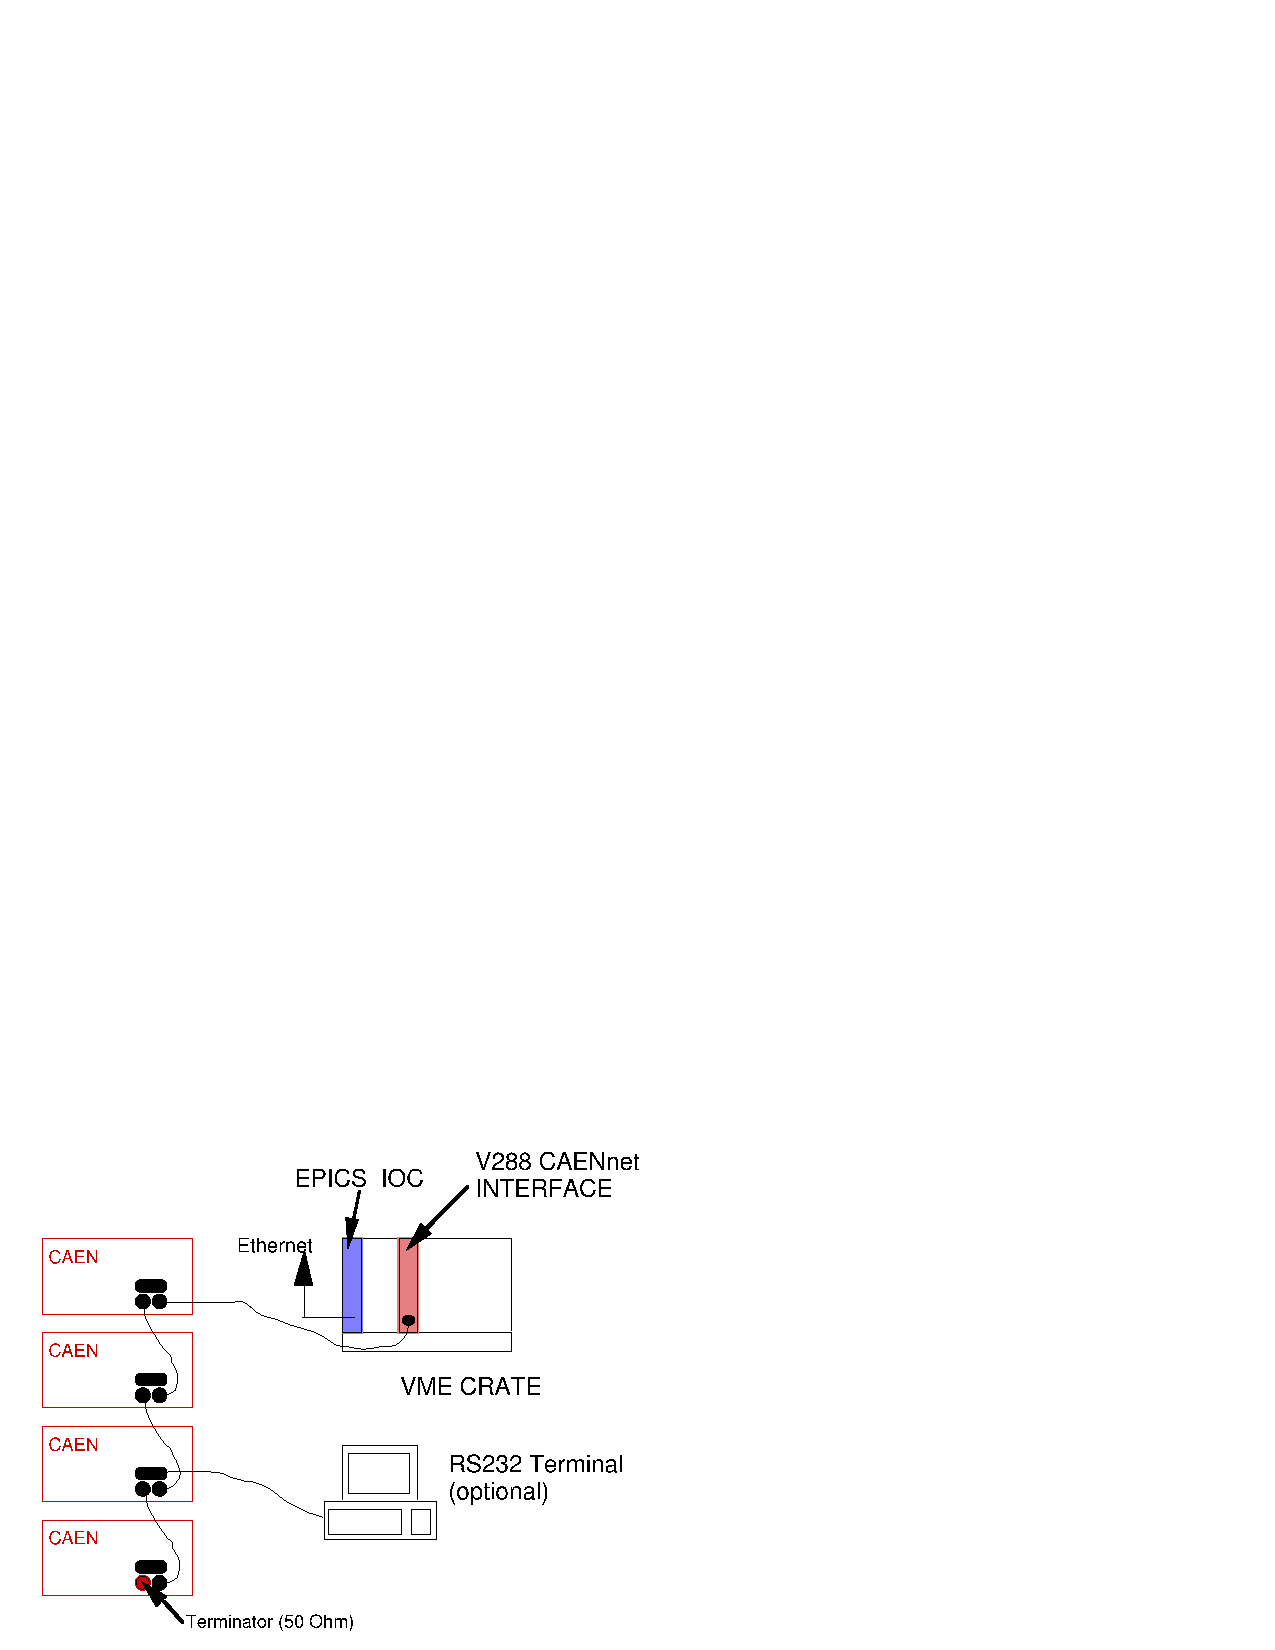
\includegraphics[height=4.5in]{CAENHV.pdf}
%\caption{Generic CAEN High Voltage System setup\label{fig:caen_setup}}
%\end{figure}

HV channel assignments currently in effect are indicated in 
two files (``group\_map'' and
``channel\_map'') in the directories \$EPICSHL/HV/hms\_all (for HMS) and
\$EPICSHL/HV/shms\_all (for
SHMS) when logged in as cvxwrks to one of the cdaq machines.

%\vfil\eject
\paragraph{General Operation}

\subparagraph{Normal Operation:}

In general the high voltage system will be controlled or monitored
from the counting house using the EPICS slow control system.
Operation of the EPICS graphical interfaces is described in the CAEN
HV Operation Howto~\cite{howto:CAEN_HV_operation}.

In case of a dead high voltage channel, the high voltage cable for a
given detector element can be moved 
to a spare high voltage channel, if available.  (The channel\_map
file, described above shows which channels are in use.)  Care must be
taken to always use the correct type of HV (positive vs. negative,
vs. drift chamber supply).  The procedure to make these changes is
described in the CAEN HV Operation
Howto~\cite{howto:CAEN_HV_operation}.  Any changes in HV configuration
shall be documented in the logbook.

For more complicated changes to the HV configuration, such as changing or
adding HV cards or mainframes, consult and expert and the Caen High
Voltage System EPICS Controls Expert Howto~\cite{howto:CAEN_HV_expert}.

\subparagraph{Important Features:}

The user can program several important features for individual
cards and/or channels.  The most common are:

\begin{itemize}
\item{HV limits -- 2 types including a hardware maximum (common to a
card) set with a pot on the front panel of each card and a software
maximum for each channel.}
\item{Current Trip Value -- The current over which the system will
indicate an alarm status and initiate a trip off of that channel.}
\item{Current Trip Time -- The amount of time the system will allow
the alarm condition before actually switching off that channel.}
\item{Ramp-up Value -- The number of volts/sec the voltage will ramp
to its set point upon switching on the channel.}
\item{Other Features -- See the CAEN Technical Information Manual.}
\end{itemize}

\subparagraph{Direct/Local Operation}
The SY403 mainframes may be controlled through the front panel or an
RS232 interface, while the SY4527 The high voltage main frames can be
controlled through a web interface.   These methods of control are
described in the CAEN HV Operation
Howto~\cite{howto:CAEN_HV_operation} and the vendor manuals for the
SY403~\cite{caensy403manual} and SY4527~\cite{caensy4527manual}.
These modes of control are meant for
diagnostics and testing of a detector system prior to running.

\paragraph{Safety Concerns/Caveats}

There are a number of cautions one should observe when operating
the CAEN HV equipment to avoid damage and insure proper functioning:

\begin{itemize}
\item{Use only proper SHV connectors and approved cables when
connecting equipment to the supply.}
\item{{\bf DO NOT} attach/remove HV cables when loads are present on the
channel ( a red LED above each channel indicates the presence of a
load).}
\item{Insure adequate ventilation around crates to avoid overheating
of the electronics.}
\item{Wait 2-3 minutes after switching off a crate before removal of a
HV card.}
\item{Insure proper static precautions when handling HV cards.}
\end{itemize}

For proper EPICS control operation (SY403):

\begin{itemize}
\item{Inter-crate connections must be unbroken and terminated at the
last crate at 50 Ohms.  All crates must be powered on.}
\item{Crate numbers for each crate in the chain must be distinct and
different from 0 (i.e. 1-99)}
\item{The HV Enable switch (on the front panel of each crate) must be on.}
\item{One should refrain from any local operation of crates when the
EPICS system is active.}
\end{itemize}

\subsection{The Wire Chamber Gas Mixing System}
\label{sec:chambergas}
% (BDS) Largely pulled from detailed gas_system_HOWTO document

The Hall~C wire chamber gas mixing system exists in the gas shed located
to the left of the counting house in the parking lot between the counting house
and the accelerator service building (building 96C).  The main
component of the system is a single MKS 647 menu driven 4-channel
controller that maintains the mix proportions and pressure regulation of the
gas supplied to the wire chambers.  Gas flow is
controlled by 2259c proportional mass flow control valves.  The 647 allows
the Gas Calibration factor to be altered in software, allowing the user to
change to a different gas without recalibration of the mass flow control
valves.

A temperature controlled alcohol bubbler is provided for the gas
stream.  The alcohol level in the stream is maintained by a float valve
fed from a reservoir outside the bubbler chiller. This allows the alcohol
system to be refilled without opening the system to air.  A sight glass on
the side of the reservoir allows the level to be monitored.  A bypass loop
around the alcohol system is provided should alcohol-free gas be desired,
or if the alcohol system requires maintenance.  Remote monitoring and limited
controls are provided through an EPICS display screen accessible via
\textbf{JMenu/Monticello $\rightarrow$ Hall C $\rightarrow$ Hall C Gas Shed},
or equivalent\footnote{Path to EDM file is /cs/opshome/edm/hlc/HLC\_gas\_shed.edl}.

{\bf This system operates by measuring and controlling pressure, not flow rate.
This system will work to maintain a pressure, regardless of the flow rate.
This allows the (pressure dependent) Rotameter-style flow meters to provide
a constant flow rate to detector systems.  Nevertheless, it should not be used
without appropriate pressure relief device such as relief bubblers and relief
valves.}

The manual valves used in this system are numbered on their
handles.  Those numbers are referenced in this document and in
Figure~\ref{fig:gas_mix}.
\begin{figure}
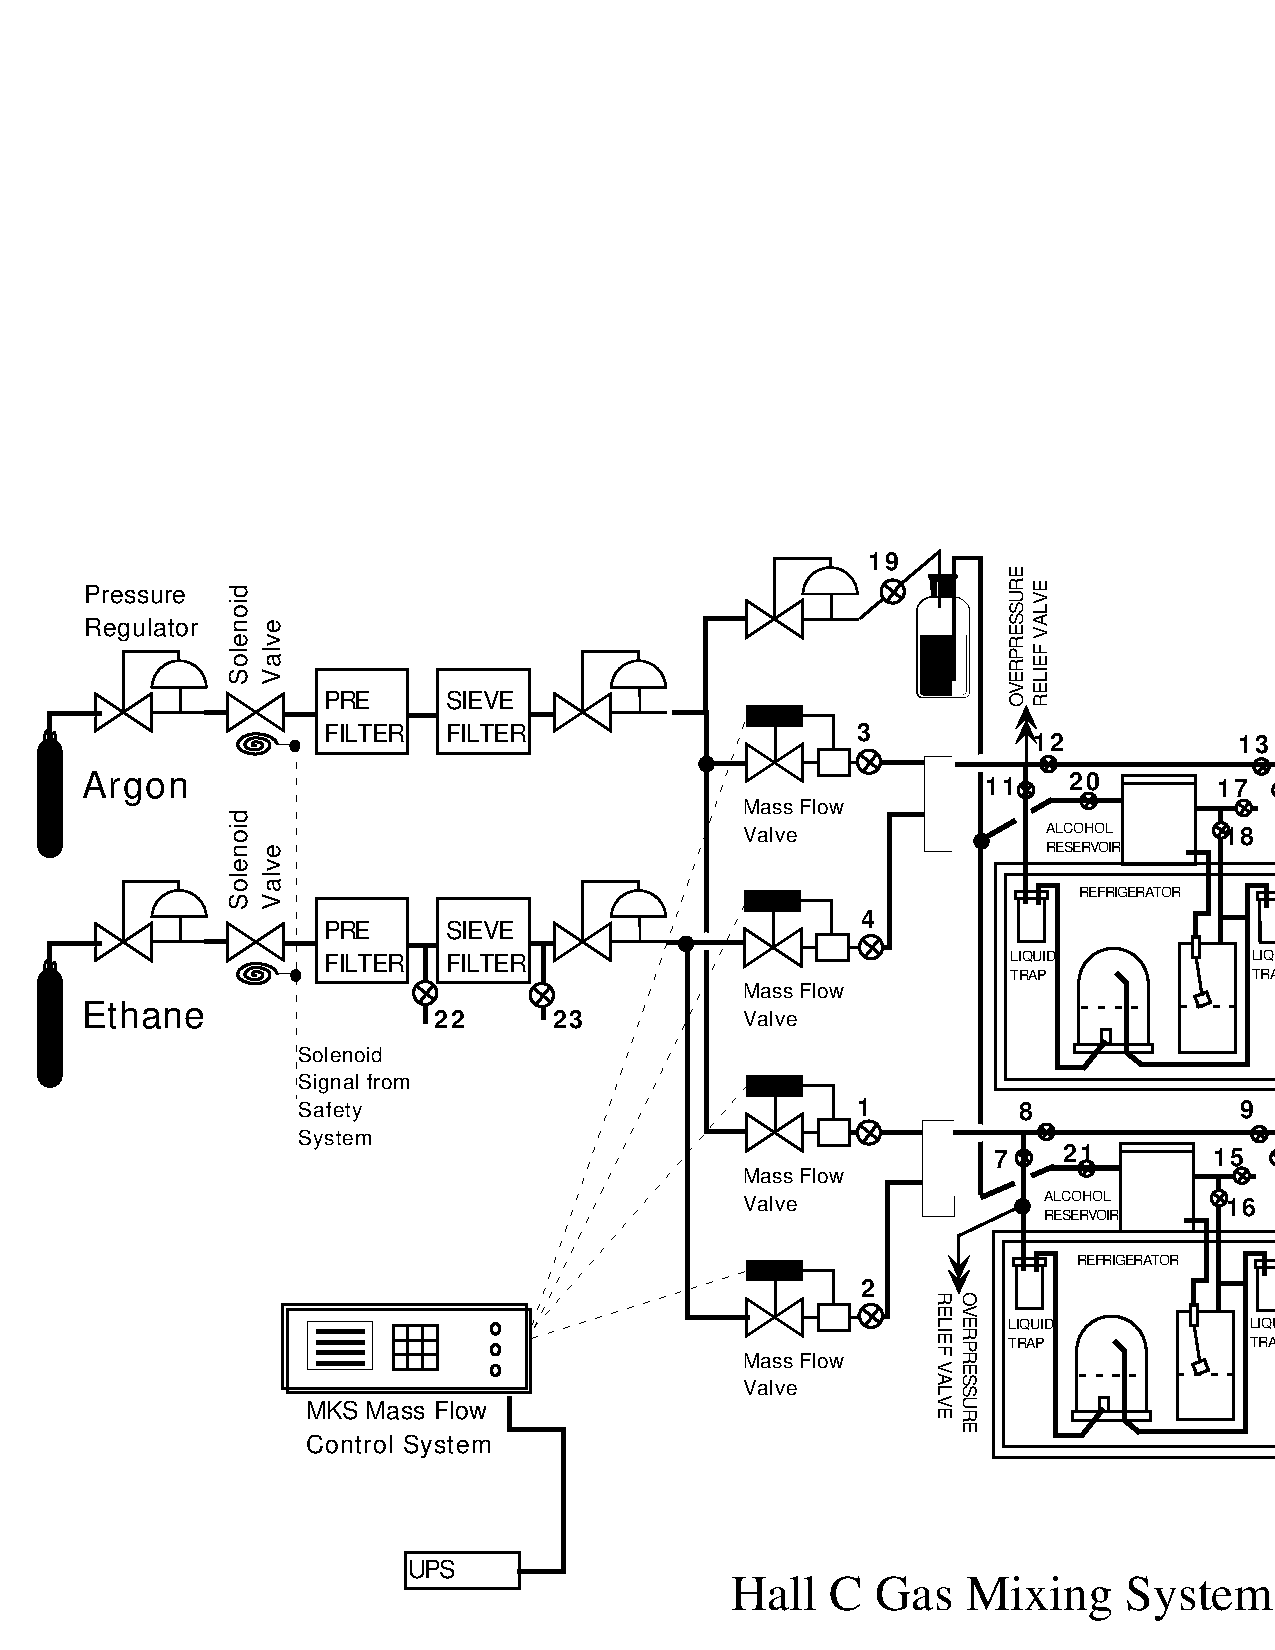
\includegraphics[width=0.9\columnwidth]{HallCGasMixlvl1.pdf}
\caption{Diagram of the Hall~C Gas Mixing System\label{fig:gas_mix}}
\end{figure}

\paragraph{Settings for Normal Operation}

A summary of all of the settings required to make the controller
function properly is given in Table~\ref{tab:mixer_nominals}. The
table also shows which screen contains each parameter. Instructions
for setting parameters are given below. Detailed instructions for
configuring and operating the MKS~647 can be found in the
manufacturer's instruction manual~\cite{647C_EN_0504A1}.

\begin{table}[hbt]
\begin{minipage}[h!]{\textwidth}
{\scriptsize
\begin{center}
\begin{tabular}{|l|c|l|}
\hline
Parameter   & Set To   & {\it Controller Screen}/Comments\\ \hline
\multicolumn{2}{|c|}{\bf Manual Valves  } &  Valves are labeled        \\
Valves 1, 2, 4, 8 & OPEN                  &         \\
Valves 3, 5, 6, 7 & CLOSED                &         \\ \hline
\multicolumn{2}{|c|}{\bf Pressure PID Loop Settings   } & {\it Pressure Control} (Fig. \ref{fig:pressure_control})  \\
Pressure    & 500 Torr &                   \\
PID Mode    & AUTO     &                   \\
PID GAIN    & 4.0      &                   \\
PID INTEG   & 10.0     &                   \\
PID LEAD    & 0.000    &                   \\ \hline
\bf Mixture     & 1        & {\it User} (Fig. \ref{fig:user_display})/ Lower-right corner\\ \hline
\multicolumn{2}{|c|}{\bf Gas Composition for Mixture 1} & {\it Gas Composition} (Fig. \ref{fig:gas_composition})\\
Channel 1   & 1.000    &  (Argon)                 \\
Channel 2   & 1.000    &  (Ethane)                 \\
Channel 3   & 0.000    &                   \\
Channel 4   & 0.000    &                   \\ \hline
\multicolumn{2}{|c|}{\bf MFC Valve Size } & {\it Range Selection} (Fig. \ref{fig:range_selection})  \\
\multicolumn{2}{|c|}{\bf  / Gas}             & {\it Gas Selection} (Fig. \ref{fig:gas_selection})  \\
Channel 1   & 2.0 SLM / Ar         & provides 2.78 SLM Argon\\
Channel 2   & 5.0 SLM / C$_2$H$_6$ & provides 2.50 SLM Ethane\\
Channel 3   & \it unused&                  \\
Channel 4   & \it unused&                  \\ \hline
\multicolumn{2}{|c|}{\bf Channels ON/OFF Settings} & {\it Extended Display} (Fig. \ref{fig:extended_display})   \\
Channel 1   & ON       &                   Press ``ON 1'' (\em Argon)  \\
Channel 2   & ON       &                   Press ``ON 2'' (\em Ethane) \\
Channel 3   & OFF      &                   Press ``OFF 3'' (\em not in use) \\
Channel 4   & OFF      &                   Press ``OFF 4'' (\em not in use) \\ \hline
\multicolumn{2}{|c|}{\bf Pressure Transducer} & {\it Pressure Setup}  \\
Controller  & STD      &                   \\ 
Range F.S.  & 1000 Torr&                   \\ \hline
\multicolumn{2}{|c|}{\bf MFC Valve Controls     } & {\it Mode Selection} (Fig. \ref{fig:mode_selection}) \\
Channel 1   & PID      &                                   \\
Channel 2   & SLAVE / 1&                                   \\
Channel 3   & INDEP    &                                   \\
Channel 4   & INDEP    &                                   \\ \hline
\bf Alcohol Temp. & 2$^\circ$\,C & Electronic Temperature  \\
                  &              & Control Box             \\ \hline
\hline
\end{tabular}
\end{center}
}%end of \scriptsize
\end{minipage}
\caption{Normal Valve and Parameter Settings for the Gas Mixing System.
\label{tab:mixer_nominals}}
\end{table}
%=====================================================================
\paragraph{General Operation of the Mass Flow Controller}
If the controller screen is dark, press {\bf ESC} to awaken the
display.  Many screens merely provide a menu of other screens you may
access: simply press the item number you desire. To go up one level in
the menu hierarchy, press {\bf ESC}. The \emph{Menu Tree} for the 647C
controller is shown in Fig. \ref{fig:command_tree}.

In general, to change a parameter displayed on the controller screen
use the \textbf{left/ right} arrow keys to move the cursor to the item you
wish to change. Then either use the number keys to enter the value
desired for that item (numeric parameter) or use the {\bf ENTER} or
{\bf up/down} keys to cycle a parameter through its available settings
(configuration parameter). Numeric parameters may be incrementally
modified by using the {\bf up/down} arrow keys. To make certain that a
new parameter becomes active, move the cursor off of the parameter
after you have entered the new value.

The initial menu upon startup is the {\bf Main Menu}
(Fig.~\ref{fig:main_menu}).  For normal operation use the {\bf User
Display} menu (Fig.~\ref{fig:user_display}). It shows the amount of
each gas currently flowing, the total gas flow, and the current
delivery pressure. This display also shows which of several possible
pre-defined gas mixtures is selected. These mixtures are configured 
on the {\bf Gas Composition} screen, Fig. \ref{fig:gas_composition}.
For normal operation, we use
only mixture {\bf \#1}, (number shown on the lower-right of the
display). {\bf Only on this screen can this parameter be changed.}
Mixture {\bf \#2} is usually configured to provide 100\% argon for
purging flammable gas out of the chambers.

The {\bf Extended Display} menu (Fig.~\ref{fig:extended_display})
shows actual flow, flow set point, units, valve full-scale range, gas
calibration factor, whether that channel is enabled, and whether each
channel is operating in master, slave, PID, or independent mode. This
display is most useful to a system expert wishing to verify the system
parameter settings.  Most parameters cannot be modified from this
screen, however.

Delivery pressure set-point and pressure \emph{PID-loop} control parameters
may be configured from the {\bf Pressure Control} screen
(Fig.~\ref{fig:pressure_control}).
%
\begin{figure}[tb]
\begin{center}
\framebox{
\begin{minipage}{.65\textwidth}
\footnotesize
\begin{itemize}
\item MAIN MENU (Fig. \ref{fig:main_menu})
   \begin{enumerate}
   \item [1] USER DISPLAY (Fig.\ref{fig:user_display})
   \item [2] EXTENDED DISPLAY (Fig.~\ref{fig:extended_display})
   \item [3] PRESSURE CONTROL (Fig.~\ref{fig:pressure_control})
   \item [4] DIAGNOSTICS
      \begin{enumerate}
      \item [4.1] ERROR LISTING
      \item [4.2] SIGNALS
      \end{enumerate}
   \item [5] INSTRUMENT SETUP
      \begin{enumerate}
      \item [5.1] RANGE SELECTION (Fig.~\ref{fig:range_selection})
      \item [5.2] GAS SELECTION (Fig.~\ref{fig:gas_selection})
      \item [5.3] MODE SELECTION (Fig.~\ref{fig:mode_selection}) 
      \item [5.4] ZERO ADJUST
      \item [5.5] TRIP LIMITS
      \item [5.6] GAS COMPOSITION (Fig.~\ref{fig:gas_composition})
      \end{enumerate}
   \item [6] SYSTEM SETUP
   \item [7] PRESSURE SETUP 
   \item [ ]
   \item [9] INFORMATION
   \item [0] POWER OFF
   \end{enumerate}
\end{itemize}
\end{minipage}
} %%end of \framebox{
\caption{Command Tree for the MKS-647C Control Panel}
\label{fig:command_tree}
\end{center}
\end{figure}
%
\begin{center}
\begin{figure}[hbt]
\begin{minipage}{2.7in}
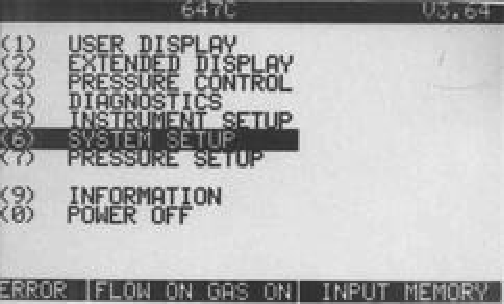
\includegraphics[width=2.6in,height=1.8in]{drift_gas_system-main_menu-eps-converted-to.pdf}
\caption{MKS~647 Main Menu\label{fig:main_menu}}
\end{minipage}
\begin{minipage}{2.7in}
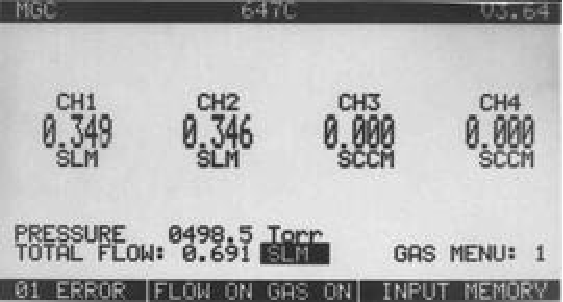
\includegraphics[width=2.6in,height=1.8in]{drift_gas_system-user_display-eps-converted-to.pdf}
\caption{MKS~647 User Display\label{fig:user_display}}
\end{minipage}
\end{figure}
\end{center}
%
\begin{center}
\begin{figure}[hbt]
\begin{minipage}{2.7in}
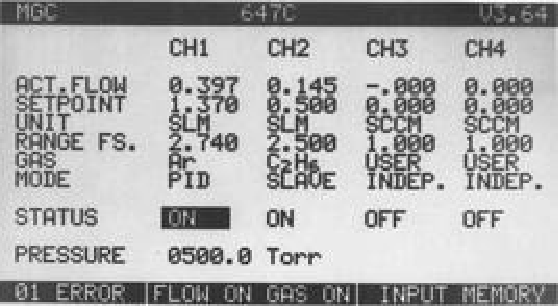
\includegraphics[width=2.6in,height=1.8in]{drift_gas_system-extended_display-eps-converted-to.pdf}
\caption{Extended Display Screen\label{fig:extended_display}}
\end{minipage}
\begin{minipage}{2.7in}
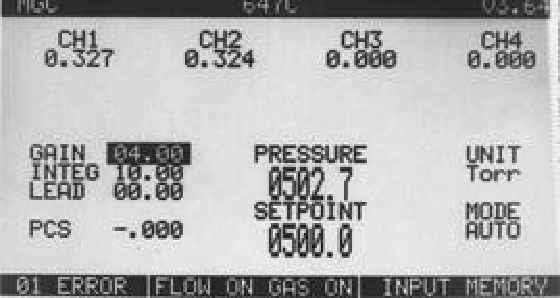
\includegraphics[width=2.6in,height=1.8in]{drift_gas_system-pressure_control-eps-converted-to.pdf}
\caption{Pressure Control Screen\label{fig:pressure_control}}
\end{minipage}
\end{figure}
\end{center}
%=====================================================================
\paragraph{Gas Flow Rates}
\label{sec:gas_flow_rates}
The flow rates are adjusted automatically by the controller in order
to maintain a constant delivery pressure at the output. Only the flow
{\em ratios} should be set by the operator. We use a 1:1 ratio, set on
the {\bf Gas Composition} screen (Fig.~\ref{fig:gas_composition}), as
indicated in Table~\ref{tab:mixer_nominals}.

The average total flow should equal the sum of the flows to all of the
detectors in the shield house. (Note that the ball-type flowmeters in
the shield house are calibrated for nitrogen. The approximate
multiplier to convert these readings for 50/50 Argon-Ethane is 0.9 .)

System configuration parameters specifying the full-scale flow
capacity (for nitrogen) of each valve, the types of gases actually
flowing through each valve, and the mode of control for the valves are
set in the screens pictured in Figs.~\ref{fig:range_selection},
\ref{fig:gas_selection}, and \ref{fig:mode_selection}. These figures
show the nominal settings for the Hall-C system.

\begin{center}
\begin{figure}[hbt]
\begin{minipage}{2.7in}
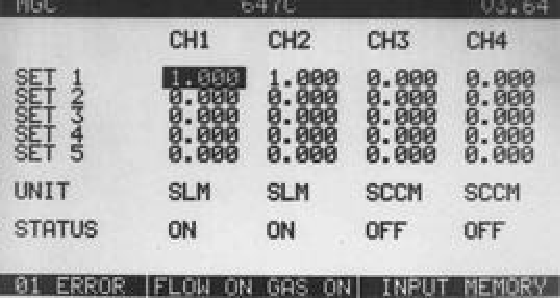
\includegraphics[width=2.6in,height=1.8in]{drift_gas_system-gas_composition-eps-converted-to.pdf}
\caption{Gas Composition Screen\label{fig:gas_composition}}
\end{minipage}
\begin{minipage}{2.7in}
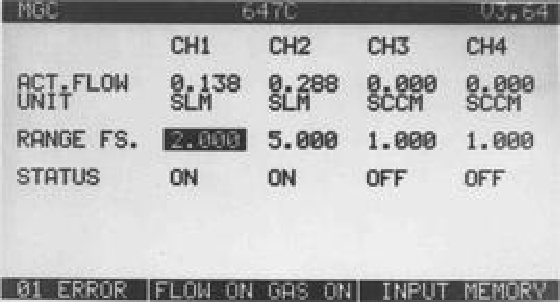
\includegraphics[width=2.6in,height=1.8in]{drift_gas_system-range_selection-eps-converted-to.pdf}
\caption{Range Selection Screen\label{fig:range_selection}}
\end{minipage}
\end{figure}
\begin{figure}[hbt]
\begin{minipage}{2.7in}
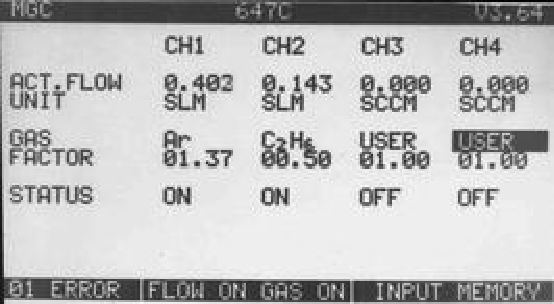
\includegraphics[width=2.6in,height=1.8in]{drift_gas_system-gas_selection-eps-converted-to.pdf}
\caption{Gas Selection Screen\label{fig:gas_selection}}
\end{minipage}
\begin{minipage}{2.7in}
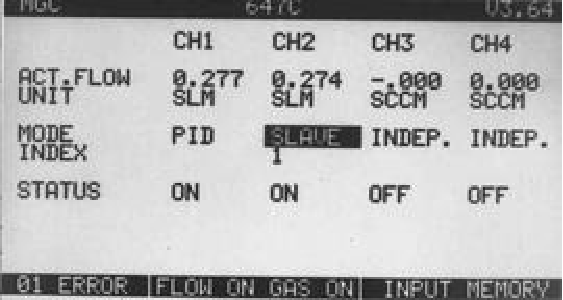
\includegraphics[width=2.6in,height=1.8in]{drift_gas_system-mode_selection-eps-converted-to.pdf}
\caption{Mode Selection Screen\label{fig:mode_selection}}
\end{minipage}
\end{figure}
\end{center}

%=====================================================================
\paragraph{To set the Delivery Pressure:}

Navigate to the {\bf Pressure Control} menu. The pressure set-point (in
Torr) is indicated at the bottom-center of the screen. This value
should be set to 500.0. Note that the system can not respond instantly
to a change in requested gas pressure: it has no way to release excess
pressure and must wait for the detector systems to consume it
\footnote{An \emph{over-pressure relief valve} releases gas through a
small oil bubbler in the gas shed if the pressure exceeds about
600~Torr.}; it cannot build up pressure any faster than the
flow-control valves can supply it. It may take thirty minutes or so
for the pressure regulation system to stabilize at a new set-point or
stabilize in response to a change in total gas consumption. However,
you should be able to observe a change in the gas flow within a few
seconds (possibly up to a minute) after a set-point change.

%=====================================================================
\paragraph{To turn gas flow on or off:}

The gas flow can be turned on or off while in any menu.  In the
Extended Display menu the bottom line displays ``ON'' or ``OFF'', by
channel, to show which mass flow valves are enabled.  ``ON'' must be
displayed in the bottom row of the Extended Display menu for gas to be
flowing in a particular channel.

For gas to flow, two conditions must be met: 
\begin{enumerate}
\item Each channel (1 and 2) must be enabled by pressing ``ON'' and then the
  desired channel number.
\item The entire system must be enabled by pressing ``ON" and then ``ALL" from
  the keypad.
\end{enumerate}
Thus, each valve can be controlled individually using ``ON/OFF~-~\emph{Channel
Number}'', or all flow can be controlled using ``ON/OFF~-~ALL''. If the system
is enabled, the status line at the bottom of every screen will indicate ``FLOW
ON GAS ON''. {\bf Note:} because Valve-2 (ethane) is normally slaved to Valve-1
(argon), when Valve-1 is disabled there will be no flow through Valve-2.

%=====================================================================
\paragraph{To Change a Gas Bottle}

Only authorized personnel are permitted to change gas bottles.

The argon and ethane supply bottles should be replaced by new (full)
bottles when the bottle content drops below about 10\% of its
capacity.  For argon, the bottle content is directly indicated by the
bottle pressure: a new bottle usually contains 2000 to
3000~psig. Argon bottles should be changed whenever the bottle
pressure is found to be below about 200~psig. 

Ethane bottles, on the
other hand, contain liquefied ethane. Thus the bottle pressure is just
the vapor pressure of ethane at whatever the current temperature
happens to be. At 70$^\circ$\,F this is about 544~psig. The pressure gauge
will not tell you how much ethane is left in the bottle until it reads
zero! Instead, we measure the ethane content by observing the weight
of the bottle and comparing it to the weight when the bottle was
full. A standard B-size cylinder contains about 32~pounds of ethane.
The ethane cylinders on the manifold sit on scales which have been 
pre-set to indicate the net weight of ethane in the bottle.
Numbers in the green portion of the dial indicate ethane remaining.
If the indicator points to the red portion of the dial, the bottle
is empty.

Handling and connecting bottles of compressed gas require special
knowledge.  The high pressure gas stored in the cylinders (bottles)
constitutes significant stored energy. Mishandling of a gas bottle can
pose a lethal hazard! Refer to the JLab ESH\&Q Manual
for safe handling practices. If you do not already know how to safely
manipulate compressed gas hardware, have a knowledgeable person train
you.

After attaching a new gas bottle to the supply manifold, check the
connection for leaks using \emph{Snoop} or a similar leak detector.

%=====================================================================
\paragraph{The Alcohol Bubbler}

To reduce the rate of aging of the wire chambers, the operating gas
contains a small quantity of alcohol vapor. The vapor is added by
bubbling the argon/ethane mixture through liquid alcohol. The
temperature of the alcohol controls the alcohol vapor pressure, which
determines the amount of vapor added to the gas. The alcohol content
also affects the electron drift velocity in the wire chambers, so it
must be held approximately constant.

Gas is bubbled through the liquid alcohol inside the glass
dome vessel in the refrigerator. The dome is covered by a
perforated steel cylinder as a precaution against breakage. The
alcohol level is controlled by a float valve inside the metal cold
reservoir, which is also inside the refrigerator. As long as there is
alcohol in the warm reservoir (sitting on top of the refrigerator),
the liquid levels inside the refrigerator will remain constant. A
drain valve (\#7) inside the refrigerator is available for emptying
all liquid from the system.  It is for use by experts only and should
remain closed during normal operation.

%=====================================================================
\subparagraph {Alcohol Temperature Control}

To keep the alcohol temperature (and thus the vapor pressure) constant,
the alcohol bubbler is housed in a refrigerator which is controlled by
an electronic temperature regulator having 1$^\circ$C sensitivity. The 
controller is located on a shelf in the right-hand rack of the gas mixing
system. Normally, the actual temperature in the refrigerator is
indicated on the front panel of the controller. The controller should
be set to maintain a temperature of 2$^\circ$\,C.

%=====================================================================

\section{Hall~C Spectrometer Magnets}

The basic parameters describing the magnets of the HMS and SHMS are provided in
Table~\ref{tab:magnet_parameters}.

The quadrupoles determine the focusing properties of the spectrometers
and to a large extent their acceptance.
To achieve the lowest possible scattering-angle
settings for each spectrometer, both Q1's are
made asymmetric: narrow horizontally and elongated in the vertical direction. For the same
reason a notch is present in the outer mantles of both Q1 vacuum cans so
that the incident electron beam passes through this notch when the
spectrometer is at its smallest angle ($12.5^{\circ}$ for HMS and $5.5^{\circ}$ on the SHMS).

In order to reach such a small scattering angle, the SHMS is equipped with the HB
(horizontal bend) dipole magnet. It bends the central-ray tracks $3^{\circ}$ away from the
beamline so that the remainder of the spectrometer components are aligned $8.5^{\circ}$
from the beam when the spectrometer is rotated to center on a $5.5^{\circ}$ scattering angle.
When used at scattering angles below about $12^{\circ}$, the stray magnetic fields from
the SHMS HB, Q1, and Q2 magnets can deflect the primary electron beam, possibly
causing it to miss the beam dump, unless the schemes designed to prevent this are followed.

The main dipole is the dispersive element in each spectrometer system. It
determines the central momentum of the spectrometer.
%The present operations envelope states that the HMS dipole power supply may not be
%operated at currents above 1300 Amps. This corresponds to a central
%momentum of about 4~GeV/c.



\begin{table}
  \begin{center}
    \caption{Characteristics of the SHMS Magnets\label{tab:magnet_parameters}}
    %\vspace{\baselineskip}
    \resizebox{\textwidth}{!}{%
      \begin{tabular}{|l|c|c|c|c|c|r|r|r|r|}
        \hline
	&		&		&			&\multicolumn{4}{|c|}{Values at Maximum Momentum}		\\
	&     		& Eff. Len.	& Aperture	&\multicolumn{1}{|c|}{Mom.}	&\multicolumn{1}{|c|}{Current}	&\multicolumn{1}{|c|}{Field or}	&\multicolumn{1}{|c|}{Energy}\\
	&     		&(m)		& (cm)		&\multicolumn{1}{|c|}{(GeV/c).}	&\multicolumn{1}{|c|}{(A)}		&\multicolumn{1}{|c|}{Gradient}	&\multicolumn{1}{|c|}{(MJ)}\\
        \hline
        HMS Q1	& Cold Iron	& 1.89	& $\phi~40$	&7.4		& 980	&	& 0.23	\\
        HMS Q2	& Cold Iron	& 2.10	& $\phi~60$	&7.4		& 830	&	& 0.81 \\
        HMS Q3	& Cold Iron	& 2.10	& $\phi~60$	&7.4		& 370	&	& 0.16	\\
        HMS D	& Wam Iron	& 5.26	& $42 (w)$	&7.4		&3000	&2.03~T	& 9.9	\\ \hline

        SHMS HB	& ``C" Septum	& 0.752	& $14.5 \times 18$	&11	& 3930	&2.56~T	& 0.2		\\
        SHMS Q1	& Cold Fe		& 1.86	& $\phi~40$	&11		&2455	&7.9~T/m	& 0.39	\\
        SHMS Q2	& $cos(2\theta )$& 1.64	& $\phi~60$	&11		&3630	&11.8~T/m& 7.6	\\
        SHMS Q3	& $cos(2\theta )$& 1.64	& $\phi~60$	&11		&2480	&7.9~T/m	& 3.4	\\
        SHMS D	& $cos(\theta )$& 2.85	& $\phi~60$	&11		&3270	&3.9~T	& 13.7	\\ \hline
      \end{tabular}
    }
  \end{center}
\end{table}

\subsection {Magnet Cryogenics}

The HMS and SHMS magnets are all
superconducting and hence their coils must be maintained at
cryogenic temperatures during operations. The LHe required by the magnets
is supplied by the End Station Refrigerator, ESR.
All of the spectrometer cryogenic services are supplied through the overhead
cryogenic lines. The distribution network begins at the distribution
box over the pivot. This box is connected to the HMS and SHMS networks via the
flexible transfer lines over the pivot. The network is adjacent to
the upstairs catwalk on the HMS and, on the SHMS, is along the small-angle side
of the upper platform.

Cryogenic information about each magnet is available on the control
screens located in the Hall~C counting house.

All of the magnets were originally designed to be cryostable, meaning that they
cannot quench unless the level of liquid helium drops below the coils. Testing of
the HMS magnets up to 4~GeV/c settings has shown that this design goal
was achieved. Nevertheless, the energy stored in the field of each magnet is sufficient
to cause an unrecoverable quench if all of it were dumped into the magnet.
Therefore, every superconducting spectrometer magnet in Hall~C, even though
cryostable, is protected by a quench protection circuit. This circuit safely dissipates
much of the magnetic-field energy in a high-power dump resistor. The SHMS
magnets have not received extensive cryostability testing yet.

\subsection {Magnet Power Supplies}

The power supplies for the magnets are located on the carriage
adjacent to the magnets. The supplies are all water cooled and
the water flow rate to the supplies can be seen on the water flow
meter located near the electronics boxes on the floor near the pivot.
This meter views the flow for all the HMS power supplies
(dipole and quads) and a reading of 33 $\%$ corresponds to approximately
20 gallons per minute through the combination of supplies (they are supplied
in parallel).
As of writing, the total flow rate for the SHMS power supplies has not been
measured. When it is measured, the nominal value will be available in the Hall-C electronic log book
and the manual you are reading will be updated.

The front panels of the power supplies are interlocked. Under
no circumstances should the front panel of any supply be opened by anyone other
than authorized personnel.

When the supplies are energized there are flashing red lights  and
illuminated "Magnet On" signs placed at
several locations on the HMS and SHMS carriages to alert personnel to the magnet
status. There are also signs posted listing the dangers of high magnetic
fields.

The control interfaces for the power supplies are available in the
Hall~C counting house on the HMS and SHMS control screens. Experimenters
use these screens to control the magnet power supplies. The magnet experts
will sometimes use controls that are local to the power supplies.

\subsection {Magnet Personnel}
In the event that any problems arise during operations of the magnets
of either the HMS or the SHMS,
one of the qualified responsible personnel listed in
Table~\ref{tab:spec:personnel_technical} should be consulted.  This includes any prolonged
or serious problem with the source of magnet cryogens (the ESR).
On the weekend and after hours there
will be a designated individual on call for magnet services. This person should be
contacted first.


%\subsection{Quadrupole Magnets}
%
%The quadrupoles determine the transverse focusing properties of the spectrometers
%and to a large extent their acceptance.
%
%All three quadrupoles for the HMS spectrometer are cold iron superconducting
%magnets. The soft iron around the superconducting coil enhances the field at
%the coil center and reduces stray fields.
%The basic parameters for the first quadrupole, Q1, are an effective (actual)
%length of 1.89 (2.34) meter and an inner pole radius of
%25.0 centimeter. \cite{bi:yan1}
%The vacuum vessel
%inner radius for Q1 is 20.05 cm. To achieve the lowest possible angle
%setting of the HMS spectrometer (with respect to the beam line), Q1 is
%made asymmetrical, and is elongated in the vertical direction. For the same
%reason a notch in the outer mantle of the Q1 cryo vessel is made, such
%that the incident electron beam passes through this notch when the
%HMS spectrometer is at its smallest angle of 12.5 degrees.
%The other two quadrupoles, Q2 and Q3, are essentially identical with an
%effective (actual) length of about 2.10 (2.60) meter and an inner pole radius
%of 35.0 centimeter. For these quadrupoles the vacuum vessel inner radius
%amounts to 30.0 centimeter.
%
%% These will need to be updated for whatever max momentum we certify
%The maximum operating currents (assuming a 4 GeV/c momentum particle) for the
%quadrupoles are about 580 A, 440 A, and 220 A, for Q1, Q2, and Q3, respectively.
%To establish a correct focusing onto the detector plane with
%the quadrupole triplet we may want to cycle the quadrupoles to about 20\% higher
%current values, rendering maximum currents of 700 A, 530 A, and 270 A,
%respectively. This will render pole field values of 1.25, 1.30, and 0.65 T,
%respectively.
%The energy stored in the quadrupole fields is sufficient to cause an
%unrecoverable quench if all the energy stored is dumped into the
%magnets. \cite{bi:hms1}
%Therefore a quench protection circuit is incorporated. However, a quench
%can only happen if the cryomagnets have a helium level below the coil during
%operation.
%
%The operating current to the quadrupole coils is provided by three
%Danfysik System 8000 power supplies, which can operate up to 1250 A current
%and 5 V voltage. The power supplies are cooled with a combined maximum
%water flow of 45 liters per minute.
%
%In addition to the main quadrupole windings, all quadrupoles have multipole
%windings to make corrections to the fields.  These mulitpole windings
%are no longer used and are not connected to power supplies.
%%To further optimize focusing properties of the HMS magnet system
%%we may operate some of these multipole trim coils
%%\cite{bi:yan2}.
%%The operating current for these multipole
%%corrections is small (the multipole corrections are typically less than
%%2\% of the main quadrupole field), of order 50 A, and are provided by
%%three HP power supplies. These power supplies can operate up to 100 A current
%%and 5 V voltage.
%
%%%
%
%\newpage
%\subsection{Dipole Magnet }
%
%The dipole is the dispersive element in the system and
%determines the central momentum of the spectrometer.
%The present operations envelope states that the supply may not be
%operated at currents above 1300 Amps. This corresponds to a central
%momentum of $\approx$4 GeV/c.
%
%The dipole for the HMS spectrometer is a superconducting, cryostable magnet.
%Its basic parameters are an effective length of 5.26 meter,
%a bend radius of 12.06 meter, and a gap width of 42 cm.
%Its actual size is 5.99 meter long, 2.75 meter wide, and 4.46 meter high.
%It is configured to achieve a 25 degree bending angle for 4 GeV/c momentum
%particles at a central field excitation of 1.11 T.
%For the HMS dipole to reach 1.11 T the maximum operating current for the coil
%amounts to 1300 A.
%
%The dipole has been designed to achieve cryostability up to a field of 2 T,
%and this property has been extensively tested up to a field of 1.11 T.
%The cryostable coils are equipped with an energy removal circuit to cover
%the possibility of an unrecoverable quench. \cite{bi:hms2}
%However, this can only happen
%if the helium level drops below the coil during operation.
%The current to the coils will be provided by a Danfysik System 8000 power
%supply, which can operate up to 3000 A current and 10 V voltage.
%This power supply is located on the carriage beside the dipole, and
%is cooled with a maximum water flow of 35 liters per minute.
%The flow of the magnet cooling water is regulated by flow meters installed
%on the floor of Hall~C. The total water flow needed to cool the 4 power
%supplies for the HMS magnet system (dipole and quadrupoles) amounts
%to 80 liters per minute, with a supply pressure of cooling water for
%Hall~C of 250 psi.


\subsection{Operation of the Spectrometer Magnets}
\label{ssec:operatemagnets}

HMS and SHMS magnet controls have been extensively revised. See
section~\ref{sec:spectrometercontrols}
for instructions. The controls and
monitoring screens are accessed through a GUI/HMI that magnet system
experts will have initialized in the Counting Room.

The information immediately following is being temporarily retained and is likely
covered in more detail elsewhere.

\subsubsection{Setting Magnet Currents}

The polarities of the currents in the HMS and SHMS magnets are such that
HB, Q2 and DIPOLE have the same sign as the charge of the particles
to be transmitted. Q1 and Q3 have the other sign. If you use the ``standard
tune" setting on the controls GUI this will be handled for you automatically.

While in the past users of Hall~C had to run a program called ``field" to obtain
the predicted current or field settings for a given spectrometer momentum,
these parameters are now determined for you by the controls program. You
need only to enter the desired momentum in the GUI.

One thing has not changed:
\begin{itemize}
\item{Wait at least 7 minutes for the HMS dipole magnet to settle.}
\end{itemize}

Up to this moment we have not witnessed any clear signature of hysteresis
effects for the HMS dipole magnet. For the HMS quadrupole magnets a small effect
on the field has been witnessed, but only for low currents (typically smaller
than 100 A). A procedure for setting the quadrupoles was developed
and shown to achieve a high
degree of reproducibility in setting the quads at low current.
\\
\\
\textbf{The HMS Quadrupole Cycling Procedure:}
\begin{enumerate}
\item{On every change of polarity, take the magnet up to 950 Amps
  (in the new polarity!), then down to zero before setting the
  current.}
\item{To set the current the first time after a polarity change
  go up to 200 Amps higher than the desired current,
  then down to the desired current.

  This means: to change the polarity and set the current go to 950 Amps,
  down to zero, back up to 950 Amps, and down to the desired setting.}
\item{Subsequently:
  \begin{itemize}
  \item{Changes to lower currents can be made directly.
    That is, just set the magnet for the lower current.}
  \item{For changes to higher current, first overshoot
    by 200 Amps, then come back down to the desired current.}
\end{itemize}}
\end{enumerate}
This procedure is called \textbf{CYCLING THE MAGNET}, and needs to be  followed for all three HMS quadrupoles.

Commissioning of the SHMS magnets with beam has not occurred as this is written, although it
is expected that only SHMS Q1 might need to by cycled. The other SHMS magnets have
current-dominated fields (rather than iron-dominated) and are not expected to
exhibit significant hysteresis effects. Cycling procedures, if needed, will be established by
the Physics Division Liaison in consultation with the engineering group and collaborators.

\subsubsection{Checking Cryogenics}

\begin{description}
\item{\bf 1}\hskip0.1in Routine checking
\item{}\hskip0.3in The HMS and SHMS magnets all operate with liquid-level controlled
  reservoirs. It is therefore sufficient to verify that the liquid level
  is near the set point to be assured of cryogenic happiness.
\end{description}

\begin{description}
\item{}\hskip0.3in The setpoints are all 70\%.  The liquid
  level is normally within a few percent of this value.  If
  the helium level is significantly above this
  the helium reservoirs are overfilling.  This is not harmful and the
  levels will return to normal in several hours.  If the level is
  significantly below the set points (5\% or more) there is usually
  something wrong.  Selecting a time graph of liquid level is helpful in
  determining if the situation is a temporary fluctuation or if the
  situation is serious.
\item{\bf 2}\hskip0.1in Helium Problem Resolution
\item{}\hskip0.3in If helium liquid level is observed falling, check the cryogen status of all nine magnet
  systems.  If multiple systems are losing liquid helium,  call CHL x7405 as the
  likely cause is a site wide problem.  CHL will advise if recovery is
  short (1-2 hours) or much longer.  If the recovery is short do nothing!
  If the recovery is long then it can be beneficial to make some
  adjustments in Hall~C.  This requires an access and a knowledgeable
  individual: the on-call Hall~C magnet responsible person
  should be summoned. Refer to Table~\ref{tab:spec:personnel_cryo}.
\item{\bf 3}\hskip0.1in Single System Failures
\item{\bf 3.1}\hskip0.1in Single System Loss of LN$_2$
\item{}\hskip0.3in If a single system is observed losing LN$_2$ you can
  wait until
  the next day to call someone in as the LN$_2$ usage of all the magnets
  is extremely low.  They can go for 24 hours without a refill. Remember that the
  HB magnet on the SHMS uses no LN2, so do not let that confuse you.
\item{\bf 3.2}\hskip0.1in Single System Loss of LHE Level
\item{}\hskip0.3in This is usually caused by a single computer failure or
  components failure.  Call the on-call magnet responsible person (Table \ref{tab:spec:personnel_cryo})
  and plan an access to Hall~C. The dipole reservoir will go empty in 1 hour so a quick reaction is
  necessary.  The quads take much longer, 4 hours or more to empty
  allowing more time to react.  All of the magnets have low level
  interlocks that will automatically safely discharge the magnets
  so that you can safely operate until they are ``dry."
\item{\bf 4}\hskip0.1in Temporary Loss of LN$_2$ To All Systems
\item{}\hskip0.3in Occasionally during site LN$_2$ delivery, the supply to
  Hall~C
  is temporarily stopped.  This can be checked by calling ESR Cryo Coordinator
  (see Table \ref{tab:spec:personnel_cryo}).  There
  can be local Hall~C problems that result in loss of LN$_2$ to the
  magnets. The ``call in" can be deferred to a convenient time for this
  kind of problem.
\end{description}

\begin{namestab}{tab:spec:personnel_cryo}{Spectrometers: magnet cryogenic experts.}{%
    In case magnet cryogenic issues, contact the Hall C
    engineer on call and the cryogenic group if necessary.
    To contact the cryogenic group during working hours, try
    David Schleeper, Joe Wilson, or the guard shack.  Outside of working hours, contact
    the guard shack at x5822 and ask for a call back from the on call cryo engineer.}
  \EngonCall{}
  \SteveLassiter{Cryo Expert}
%  \EricSun{Cryo Expert}
%  \MikeFowler{Cryo Expert}
%  \AndyKenyon{Cryo Expert}
  \CryoonCall{}
  \DavidSchleeper{ESR Cryo Coordinator}
  \JoeWilson{Cryo Operations}
\end{namestab}


%
%\begin{table}
%\begin{center}
%\caption{Current Liquid Level Settings\label{tab:liq_levels}}
%\vspace{\baselineskip}
%\begin{tabular}{|l|l|l|}
%\hline
%{} & {}  & {}  \\
%{} & LHE & LN2 \\
%{} & {}  & {}  \\ \hline
%Q1  & 75\% & 75\% \\
%Q2  & 75\% & 75\% \\
%Q3  & 75\% & 75\% \\
%Dipole& 70\% & 70\%/65\% (Hi/Low) \\
%\hline
%\end{tabular}
%\end{center}
%\end{table}
%

\infoleveqnull{\section{Vacuum Systems}}

\sawnote{This chapter is taken from the Hall A manual.  It needs to be
amended for hall C.}

The Hall A vacuum system consists of 5 separate but interconnected 
subsystems.  The largest is designed to supply 
the Hall A HRS (see Chapter \ref{chap:hrs}) with a 
self contained 5 $\times$ 10$^{-6}$ Torr vacuum that enables both 
spectrometers to be pumped down from atmospheric pressure. in a few hours.  The target 
vacuum system is designed to maintain 1 $\times$ 10$^{-6}$ Torr in 
order to minimize contamination and provide an insulating vacuum for the 
cryo target.  Rough insulating vacuum for the 4 superconducting magnets 
is provided by a 360 \emph{cfm} Roots type blower that can be connected to each 
magnet.  The beam line vacuum is maintained by 1 $\ell$/s ion pump 
system used in the accelerator ring and a small turbo pump located near 
the target.  The final subsystem is a differential pumping station 
located near the target exit port.

\infolevone{
\section{HRS Vacuum System}

The HRS vacuum system is shown in Figure~\ref{fig:hrs_vac_sys}.
Vacuum for the HRS is supplied by an Alcatel 880 $\ell$/s Turbo 
pump backed by a Balzers 360 \emph{cfm} Roots type Blower.  This Blower, via a 
special manifold, also supplies the roughing vacuum to the HRS at the 
Dipole Inlet Transition.  The first Turbo is mounted on the lower side 
of the Dipole entrance transition.  The roughing port is also located on 
this transition, on the top side.  The upper turbo is located on the 
lower side of the window transition.

Vacuum readouts and interlock outputs are supplied by five (5) HPS 
series 421 Cold Cathode gauges and seven (7) series 275 Mini-Convectron 
gauges.  In addition to these there will also be a FIsons Micromass 386 
RGA head installed in the system for diagnostic purposes.  Most of this 
instrumentation will be located on the Turbo pump manifold (for detailed 
information see Figure~\ref{fig:hrs_vac_sys}).

\begin{figure}
\begin{center}
%\includegraphics[angle=0,width=15cm]{fig0125new}
{\linespread{1.}
\caption[Spectrometers: HRS Vacuum System]{HRS vacuum system.}
\label{fig:hrs_vac_sys}}
\end{center}
\end{figure}

Powered valves, instrumentation and pumps will be controlled and powered 
at the Vacuum System equipment rack located on each respective 
spectrometer on the gantry platform.  Selective equipment will also be 
controllable from the Hall A counting house.

{\bf Chamber}

The HRS vacuum chamber consists of an associated vacuum window, a sieve 
slit and Q1 transition, Q1 to Q2 transition, Spool section, Dipole 
transition, Dipole to Q3 transition, and the Q3 to exit window assembly. 
 The spectrometer vacuum is contained by a 0.007 inch kapton window at the
 entrance and a 0.004 inch titanium window at the exit.

\section{Target Vacuum System}

Vacuum for the target chamber is supplied by an Alcatell 880 $\ell$/s 
Turbo pump backed by an Alcatell 21 \emph{cfm} 2 stage vane pump.  The Turbo is 
mounted on the lower ring of the Target Chamber to one side so as not to 
interfere with the Target Chamber windows.

The same instrumentation is used here as on the spectrometer.

Powered valves, instrumentation and pumps will be controlled and powered 
at the Vacuum System equipment rack located on the access Balcony.  
Selective equipment will also be controllable from the Hall A counting 
house. 

\section{Magnet Vacuum System}

Vacuum for the magnet insulating vacuum is provided by the Cryo
pumping effects of each individual magnet.

All controls for the Magnets are manual as we expect no problem after 
initial pump down.


The insulating vacuum for each magnet is self contained within the 
magnet.

\section{Beam Line Vacuum System}

Vacuum for the entrance beam line is supplied by 65 $\ell$/s Balzers turbo
pumps, the first of which is located on the E P chamber, and the
second located 3 $m$ upstream of the target chamber.  Both turbos
are equipped with a HPS 7 Series 275 mini Convectron gauge and a HPS
series 421 Cold Cathode gauge located near the balcony.

Vacuum readouts and relay outputs for interlocks are supplied by HPS series 421 
Cold Cathode gauges.  In addition to these there will also be Convectron 
gauges.  Most of this instrumentation will be located on the Turbo pump 
manifold.

Powered valves, instrumentation and pumps will be controlled and powered 
at the Vacuum System equipment rack located on the Balcony.  Selective 
equipment will also be monitored from the Hall A counting house.  All 
control is by Accelerator in the MCC.

\section{Beam Exit Vacuum System}

Vacuum for the target chamber is supplied by an Alcatell 880
$\ell$/s Turbo pump backed by an Alcatell 21 \emph{cfm} 2 stage vane pump
which maintains a $1x10^{-4}$ vacuum on the exit beam pipe.

Between the target chamber and the exit beam pipe there is a 0.007 inch
kapton window that has a 0.0375 inch hole in it at the beam spot.  This
window acts as a differential pumping station.

Also between the target chamber and the exit beam pipe is an 8 inch
air actuated gate valve that is operated from the MCC.

Vacuum readouts and interlocks outputs are supplied by an HPS 7 Series 
275 mini Convectron and an HPS series 421 Cold Cathode gauge
which are located near the balcony.

Controls are interlocked to the beam.

The chamber is made of a low mass aluminum corrugated vacuum tube of 1 
$m$ diameter.

At the exit point of the exit beam pipe is a beam diffuser that
consists of 2.025 inch beryllium windows with a water filled cavity between
them for cooling.  The water is circulated through the cavity by a
water cooling system located on the Hall floor, and is interlocked
through the FSD system with 2 flow switches, one on the supply and
one on the return line.

Due to high radiation levels at the exit beam pipe all seals in
this area are metal.
} %infolev

\begin{safetyen}{0}{0}
\infolevone{\section{Safety Information}}

\subsection{Hazards}
Hazards associated with the vacuum system are due to rapid 
decompression in case of a window failure. Loud noise can cause hearing
loss.  

\subsection{Mitigations}
To mitigate the hazard, all personnel in the vicinity of the 
large chamber with a window are required to wear ear protection when
the chamber is under vacuum. Warning signs must be posted at the area.

The scattering chamber is equipped with a large 0.016" thick aluminum window that 
allows the spectrometers to swing from 12.5$^{\circ}$ to 165$^{\circ}$ 
on the left side and 12.5$^{\circ}$ to 140$^{\circ}$ on the right side. 
In order to
protect this window when the Hall is open, lexan window guards are
installed.

At the inlet of the sieve slit a 8" diameter 7 mil kapton window 
is provided to separate the target chamber from the spectrometers.
Finally, under the HRS detectors, a 4 mil titanium window is provided.  

Additionally, all vacuum vessels and piping are designed as pressure 
vessels.
\end{safetyen}

\begin{safetyen}{0}{0}
\subsection{Responsible Personnel}
\end{safetyen}
The authorized personnel is shown in Table \ref{tab:vacuum:personnel}.
\begin{namestab}{tab:vacuum:personnel}{Vacuum: authorized personnel}{%
      Vacuum in Hall A: authorized personnel. ``W.B.'' stands for the white board 
      in the counting house.}
  \TechonCall{\em Contact}
  \EdFolts{}
\end{namestab}



\section{Spectrometer Slit Systems}
\label{sec:slit}

\subsection{HMS}
\label{sssec:hms_slit}
The HMS slit system is installed on the gate valve housing mounted to the
front face of Q1. It consists of a vacuum box with a slit ladder
mounted into it. The slit ladder has space for three separate slits,
which will typically be one sieve slit and two solid angle defining collimators.
The slits are rectangular blocks of densimet (90\% W and 10\% Cu/Ni)
with a density of 17 g/cm$^3$. The collimators have an octagonal shaped
opening machined into them; the sieve slit has many holes drilled
into it.

The outer size of the collimators is 11.75" vertical by 8.25"
horizontal. The outer size of the sieve slit is 10.00" vertical
by 8.25" horizontal.
Its vertical size is reduced w.r.t. 11.75" due to space constraints.
The sieve slit always has to be installed at the bottom position of the ladder,
so that we can use the shielding of the collimator above it to
clearly distinguish the top row of holes. The central hole
of the sieve slit has a smaller aperture, and two blocked holes
exist to easily distinguish center and directions.
The collimator thicknesses are 2.5", while the sieve slit thickness
is 1.25". The dimensions and shape of the inner aperture of the present
HMS collimators is denoted in Table~\ref{tab:apertures}.

\begin{table}
\begin{center}
\caption{Apertures of Collimators\label{tab:apertures}}
%\vspace{\baselineskip}
\begin{tabular}{|c|c|c|c|c|}
\hline
{} & {} & {} & {} & {} \\
HMS & d$\Omega$ & Horizontal & Vertical & Shape \\
{}  & (msr) 	& (mr) 	     & (mr) 	& {} 	\\
{} & {} & {} & {} & {} \\ \hline
Large Collimator  & 6.74 & $\pm$ 27.5 	& $\pm$ 70.0 	& Octagonal, Flared 	\\
``Pion'' Collimator&  	& $\pm$	& $\pm$  	& Octagonal, Flared 	\\
{} & {} & {} & {} & {} \\ \hline
%SOS & 7.55 & $\pm$ 57.5 & $\pm$ 37.5 & Octagonal, Flared & \\
%SOS & 3.98 & $\pm$ 32.5 & $\pm$ 35.0 & Octagonal, Flared & \\
SHMS	& d$\Omega$ 	& Horizontal 	& Vertical 		& Shape 	\\
{} 	& (msr) 	& (mr) 		& (mr) 		& {} 	\\
Collimator &   4         & $\pm$ 24      &  $\pm$ 40     & Octagonal, Flared \\
\hline
\end{tabular}
\end{center}
\end{table}

The total depth of the slit box is close to 3.75", which leaves
enough space to later mount scintillators behind the collimators as an active
veto counter (to prevent punch-through of hadrons) and/or to increase
the collimator thickness. Two circular quick-connect flanges are
added for feed-through of possible light guides.

\subsection{SHMS}
\label{sssec:shms_slit}
A similar remotely-operated collimator box is installed on the SHMS between the
HB and Q1 magnets. The collimator ladder assembly within this box may be positioned
at three settings. The top position (accessed when the assembly is at its lowest
position) is a stretched octagon with opening height 9.843" and width 6.693" on the
upstream side. It is 2.5" thick. The lower two positions both present sieve holes in
rectangular pattern with holes separated by 0.6457" horizontally and 0.9843"
vertically. The sieve pattern at the middle ladder position has 11 columns of holes with
the sixth column centered horizontally. The holes on the bottom sieve are in ten
columns and are offset by one-half a column gap from those in the middle sieve.
The sieve collimators are 1.25" thick. The geometry is illustrated in Fig.~\ref{fig:SHMS_Collimators}.
Both sieves and octagonal collimator are
made of Mi-Tech\texttrademark{} Tungsten HD-17 (Density 17 g/cc. 90\%~W, 6\%~Ni, 4\%~Cu).

Because the SHMS has both a horizontal bend (HB magnet) and a vertical bend (main Dipole
magnet), a second sieve collimator is helpful for optics calibration and understanding the magnets.
It is placed immediately
upstream of the HB magnet entrance. Two options are provided: a conventional passive
sieve collimator and the so-called \textit{active sieve} which is a detector based on Gas Electron
Multipliers (GEMs).  A photo of the passive sieve options is shown in Fig.~\ref{fig:HB_Sieve_Photo}
and the dimensions and hole pattern are shown in Fig.~\ref{fig:HB_Sieve_Layout}.

\begin{figure}
\begin{center}
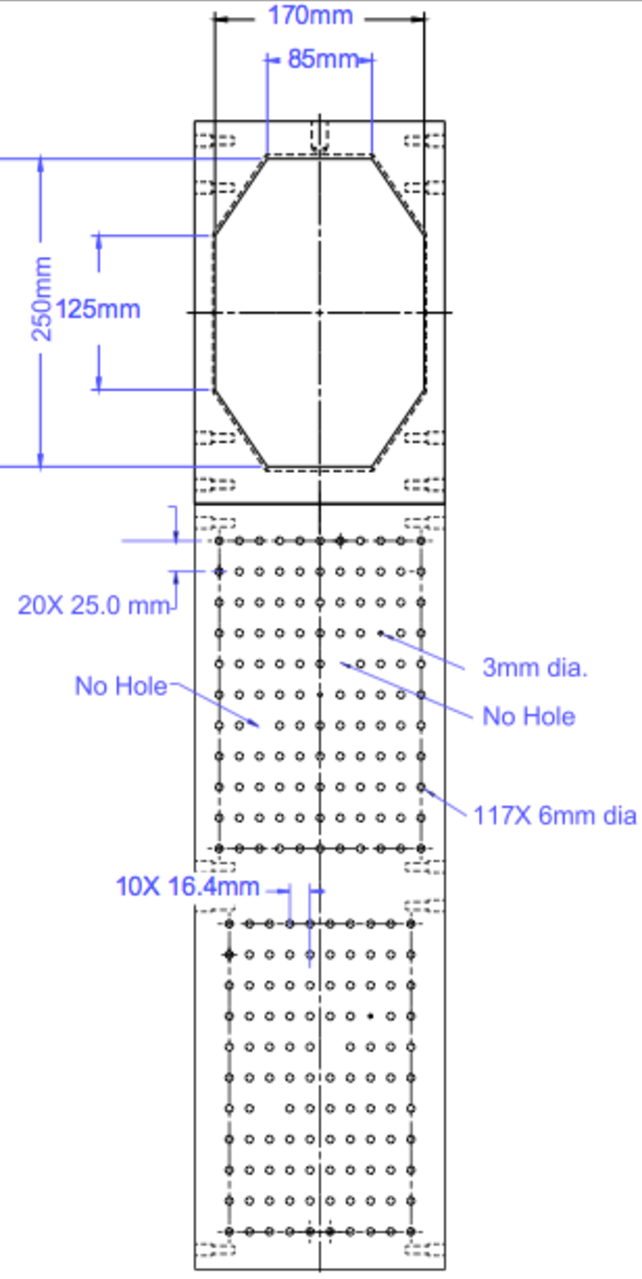
\includegraphics[width=2in]{SHMS_Collimators}
\caption{Geometry of the Main Collimator and the Sieve Slits in the SHMS \label{fig:SHMS_Collimators}}
\end{center}
\end{figure}

\begin{figure}
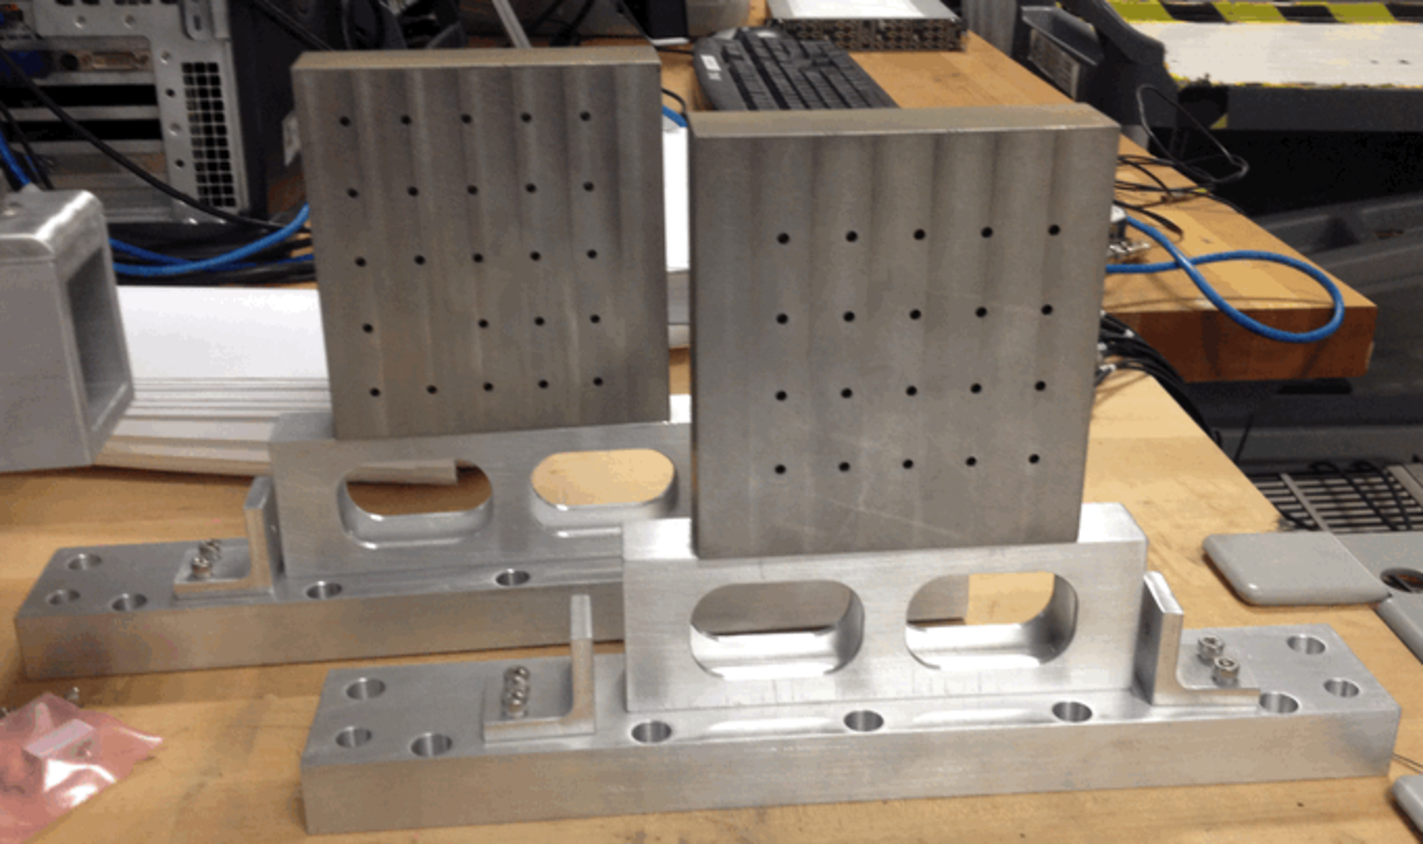
\includegraphics[width=6in]{HB_Sieve_Photo}
\caption{Upstream Sieve Slits that go on the front of the HB magnet of the SHMS \label{fig:HB_Sieve_Photo}}
\end{figure}

\begin{figure}
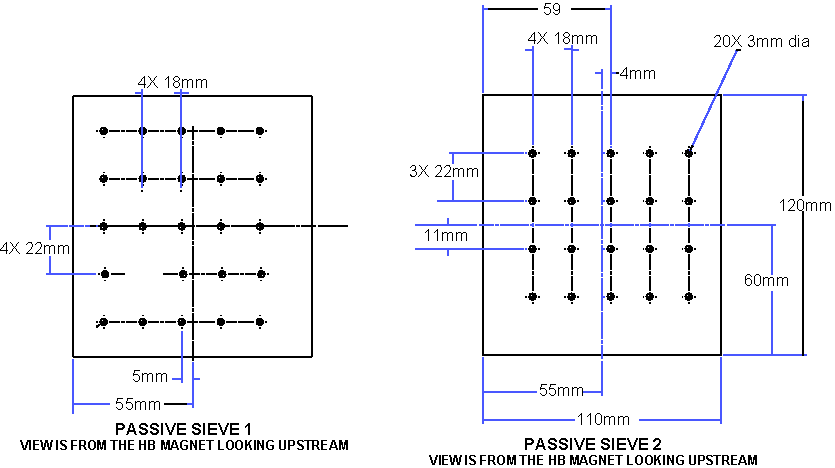
\includegraphics[width=6in]{HB_Sieve_Layout}
\caption{Upstream Sieve Slits that go on the front of the HB magnet of the SHMS \label{fig:HB_Sieve_Layout}}
\end{figure}

\subsection{Operation of the Slit System}\label{sssec:slit_control}
The HMS and SHMS slit systems are controlled by a remote control system consisting of
motor/actuators that slide the slits in place. Resolvers specify the exact position of the slits.
The resolver position of the slits is relative number of counts from the home position. The home position
is set by a homing procedure that is programmed into the controller that sets the zero position by moving the
slit to a position that activates the physical home switch. Once this homing procedure is complete, then
the slits can be moved to surveyed positions that have been programmed. The home position for HMS and SHMS slit system
does not mean that the slits are moved out of the way. For the HMS is is possible to move the slits so that
they are out of the way ({\it All Out}), but for the SHMS there is no such position for the slits.
EPICS drivers have been written for
normal operation of the slits by users and non-experts and operation of the slits through the EPICS
screens is described below. Upper and lower limit switches are on the slit system drive shaft to keep the
slits from being moved too far in either direction. There are also software limits.
The control box is located downstairs in Hall C. In the control box, there is a driver
for the HMS and one for the SHMS. If power is lost to the control box, then the brake engages
on the motor that drives the slits. On the front of the control box is
a red  emergency power shutoff button. The control box should only be opened by trained experts.

EPICS drivers have been written for normal operation of the slits by users and non-experts. The
EPICS screens are accessed through the accelerator {\bf jmenu}. Instructions for access the
  {\bf jmenu} will be given in the Hall C How-tos.
From the  {\bf jmenu}, the HMS and SHMS slit system EPICs controls can be accessed on The Hall C Operations Menu
which is open from {\bf jmenu $\rightarrow$ Standalone Menus $\rightarrow$ HallC}. On the Hall C Operations Menu under
{\it Experiment Specific} are {\it HMS Coll. Motion Control} and {\it SHMS Coll. Motion Control}. Clicking the
respective title will bring up the EPICS screens shown in Fig.~\ref{fig:normal-coll-epics}.  Fig.~\ref{fig:normal-coll-epics}
shows the HMS and SHMS slit controls in normal operation. In normal operation, the homing procedure has been completed
as indicated by the orange rectangles next to {\it Home position found/reference point point set} and {\it Home routine finished}.
With the homing procedure completed, the user can moved to the other slit positions by clicking on the labeled button. For the
HMS slit system, the slits can be moved so that they are out of the acceptance by clicking on the {\it All Out} button.
It is not possible to move the SHMS slit out of the acceptance.
\begin{figure}
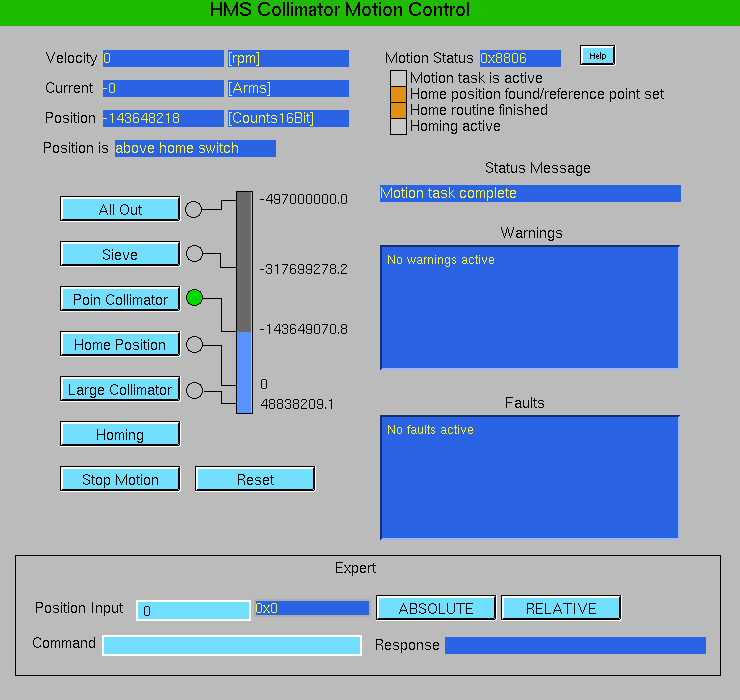
\includegraphics[width=.45\textwidth]{HMS_EPICS_pioncoll}
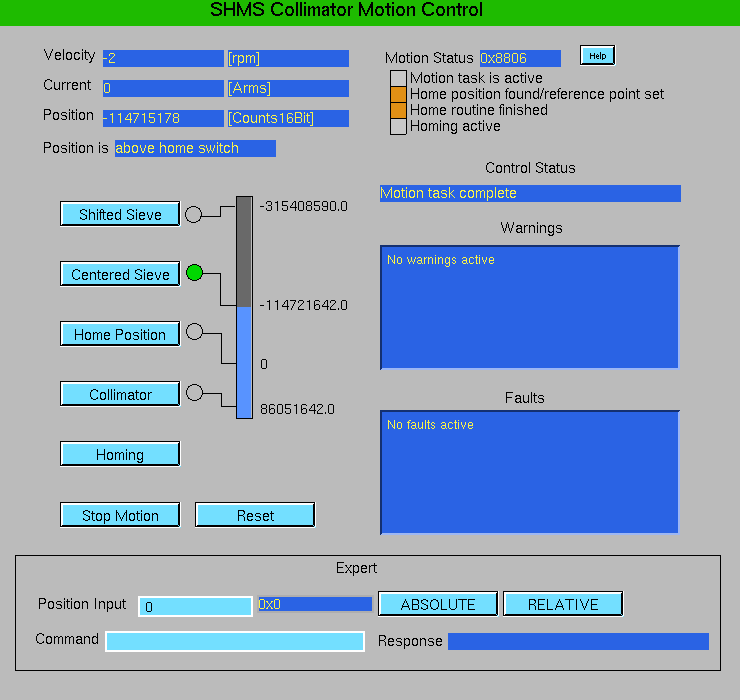
\includegraphics[width=.45\textwidth]{SHMS_EPICS_centersieve}
\caption{HMS and SHMS slit system screens in normal operation. \label{fig:normal-coll-epics}}
\end{figure}
In Fig.~\ref{fig:moving-coll-epics}, the EPICS screens are show when the slits are moving. The velocity should be around 1000 rpm and
the current less than 2 amps ( typically the reading fluctuates between 0 and 1). If the current is above 2 amps,
then click the {\it Stop Motion} button and contact the expert.
\begin{figure}
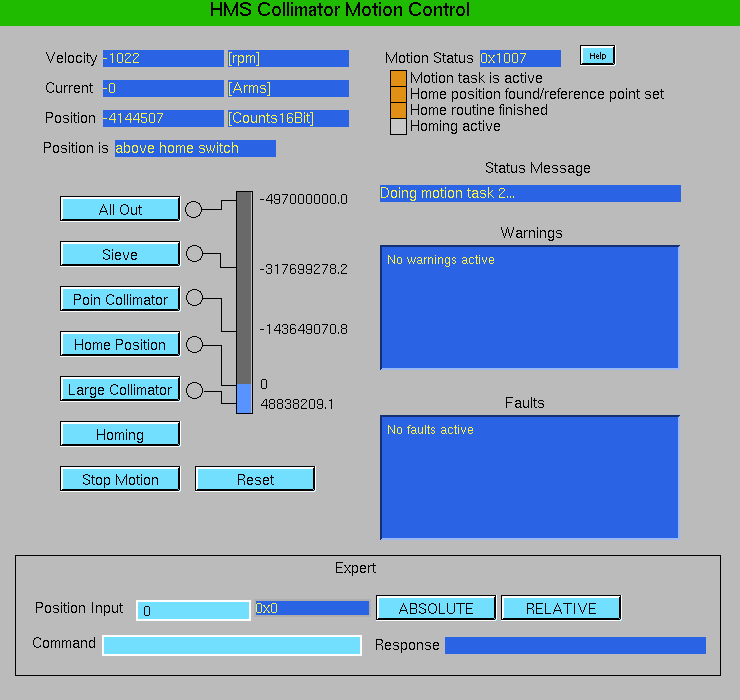
\includegraphics[width=.45\textwidth]{HMS_EPICS_moving}
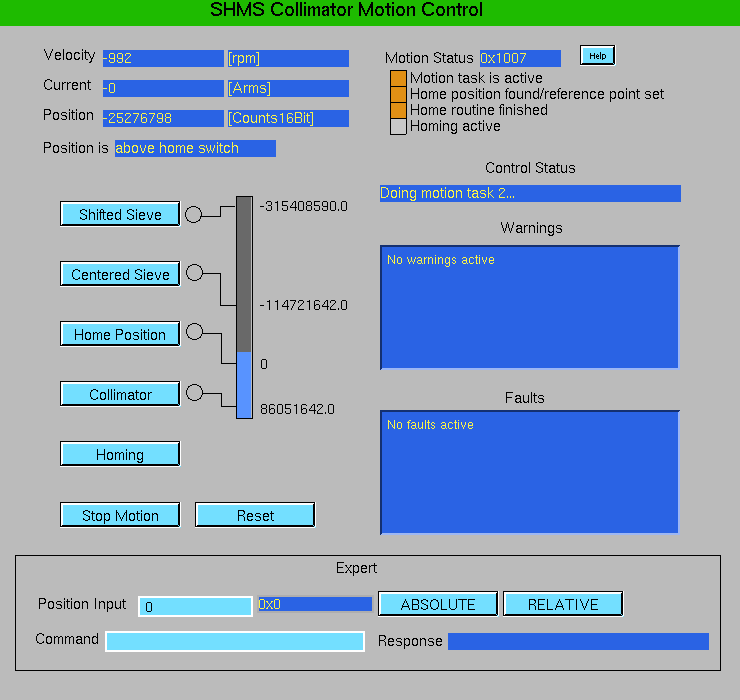
\includegraphics[width=.45\textwidth]{SHMS_EPICS_moving}
\caption{HMS and SHMS slit system screens when the slits are moving. \label{fig:moving-coll-epics}}
\end{figure}
The option of experts moving the slits to an arbitrary position
is available for the EPICS screen. The conversion is 327680 counts is one mm. The mostly likely use for this option is during the
taking of optics data when one wants data with the sieve slit moved by half the distance between holes to get more vertical angles.

The EPICS controls are done through an soft IOC called {\it  iocsofthmsco} and {\it iocsoftshmsco}. If EPICS screens are white then the IOC
needs to be rebooted. Another reason that soft IOC would need to be reboot would be if the soft IOC has lost communication with the driver.
In the case , the user could not move the slit and the text on the Warnings and Faults windows is in light grey color. Only the MCC operator can
reset the soft IOCs by accessing {\bf jmenu $\rightarrow$ Operations $\rightarrow$ Control Systems $\rightarrow$ Reboot $\rightarrow$ HallC}. The user can
call MCC to reset the soft IOCs.

If there is a power outage, the brakes are engage in the motor that drives the slits. Once power is restored then the user needs to do the
following steps to get the slit system back in normal operation mode.
\begin{enumerate}
\item Ask MCC to reboot the soft IOC for the HMS and SHMS, {\it  iocsofthmsco} and {\it iocsoftshmsco}.
\item Access the HMS and SHMS EPICS screens.
\item On the EPICS screens, click on the {\it Reset} button. this runs an initialization program which loads parameters into the driver. The EPICS screen should look like Fig.~\ref{fig:red-screen-epics}. The red warning is to remind the user to execute the homing procedure.
\item On the EPICS screens, click on the {\it Homing} button. This executes the homing program which defines the home position and is needed before moving to other position.
\item When the homing procedure is successful then the rectangles next to {\it Home position found/reference point point set} and {\it Home routine finished} will be orange.
\item Click on button to move slit to desired position.
\end{enumerate}
\begin{figure}
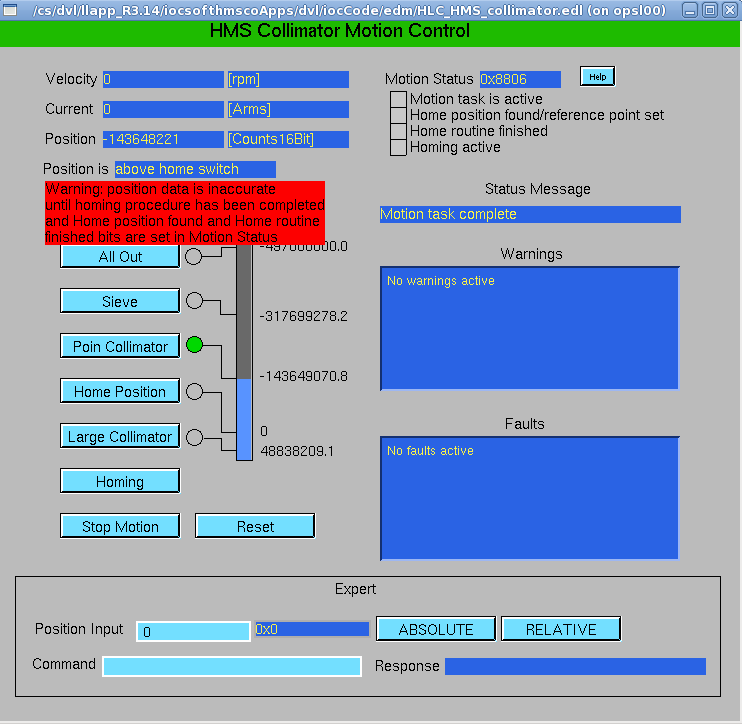
\includegraphics[width=.45\textwidth]{HMS-EPICS-red-screen}
\caption{HMS EPICS screen when power restore but before the homing procedure as been executed. \label{fig:red-screen-epics}}
\end{figure}





%\begin{table}[!ht]\
%\caption{Slit Collimator Positions\label{tab:col_pos}}
%\begin{center}
%\begin{tabular}{rlrr}
%   &                  &     HMS   & SOS\\
%\hline
%1) & Sieve Slits      &  19804600 &  11638719\\
%2) & Large Collimator &       N/A &   3190717\\
%3) & Pion Collimator  &  -3096800 &       N/A\\
%\end{tabular}
%\end{center}
%\end{table}



\subsection{Hazard Identification}

The principal hazards are:
\paragraph{Magnetic:} There is a significant fringe field at
the entrance and exits of the magnets. This represents a hazard
to people working on the slit system if they are handling magnetic
objects (tools) or to people with pacemakers. In addition the field could erase magnetic
information storage media such as the strips on credit cards.
\paragraph{Mechanical:} At the front of Q1 the housing for a spring loaded gate valve is
mounted. In its normal operation mode a metal gate will be closed with
severe pressure when the electrical power drops. This can cause serious
damage to interfering body parts.  But currently the shutter and
actuator have been removed so this hazard does not exist.
A similar mechanical problem involves the slit ladder itself. The total weight of
the three slits amounts to approximately 350 Lbs (160 Kg) and can easily
cause serious damage to body parts.

\subsection{Hazard Mitigation}

\paragraph{Magnetic}

A sign will be posted which indicates the presence of a high magnetic
field ( this is standard JLab safety signage). The exact wording is
`` High Magnetic Field - No Pacemakers or Credit Cards." There are also
flashing red lights located on the HMS and SHMS carriage indicating that the
magnet power supplies are energized. Be careful with tools (are they magnetic?)
when you work on the slit boxes with the red lights in a flashing state.

\paragraph{Mechanical}

If the gate valve is ever re-installed, the following safety
procedures should be observed.  Without power, the gate valve assumes its default closed position due to
pressured air. When installing the slit boxes, or working with your hands
in the vicinity of the inside of the gate valve, disconnect first the power
plug of the gate valve, such that the gate valve closes.
In case you need the gate valve to assume a default open position without
power, first relieve the air pressure
with power on, and verify that the default position of the gate valve has
changed to ``open" by removing the power.

When installing the slit ladder, be careful when you work with your hands
under the slit ladder (like when you are bolting the slit box to the
gate valve). Remove the slit ladder, or {\bf install a support under the slit
ladder to prevent it from falling all the way down}.

A brake system has been included in the control to prevent the slit ladder
from sliding down in case of a power failure.  However, this must not
be relied upon for personnel safety.


}
\section{Spectrometer Carriage and Rotation Systems}

The Carriage is the support structure of the spectrometer.

Each entire spectrometer can be rotated. Rotation is driven by motors mounted
near one of the sets of wheels. These motors are controlled by synchronous
pulse width modulated drives which are mounted near the bottom of the shield
house steps on the HMS, and under the rear of the SHMS structure.

\infolevone{
The spectrometer angles are found using a reference plumb bob and/or TV camera
attached at a known location under the rear of each spectrometer.
This camera is focused on survey marks scribed into plates which are attached to
the rail on the floor. Using the scribe plates and a vernier scale, the angles of the
spectrometers may be determined with a resolution of approximately $0.01^{\circ}$.
}

Since the Hall C spectrometers each weigh hundreds of
tons, it is very important that all safety precautions are carefully
adhered to.   During operations, the spectrometers are certified
to allow remote rotation by shift crews within prescribed limits.  In
the absence of this certification, the spectrometers may only be
rotated by trained technical staff.


\begin{safetyen}{0}{0}
\subsection{Hazards}

Hazards include:
\begin{itemize}
\item{Knocking items over during spectrometer movement.}
\item{The wheels crushing things (including fingers and toes) on the floor in the path of the
spectrometer}
\item{Damaging the beamline or other equipment on the floor if one goes to too small
or too large an angle.  There is
only a small gap between the rear of the SHMS shield house and the shielding wall
behind it.}
\item{Tearing out of cables etc. physically attached to the superstructure}
\item{Elevated platforms on the spectrometer carriages.}
\item{Magnetic fields.  Spectrometer magenets may be energized under either
local or remote control.}
\end{itemize}

\subsection{Mitigations}
Hazard mitigations:
\begin{itemize}
	\item{Stop-blocks attached to the rails to prevent spectrometer rotation beyond
	the needed angular range for each experiment.}
	\item{During experiments, the spectrometers are certified for rotation by
	shift crews within specied angle ranges.  Spectrometer movement at other times
	may only be performed by authorized personnel.}
	\item{Hand rails are installed to prevent falls.  Access is only allowed to
	areas on the carriage protected by hand rails.}
	\item{Hard hats may be required under certain conditions when working on or
	near the spectrometer carriages.}
	\item{Magnetic fields hazards are indicated by either red flashing lights and/or
	illuminated \textbf{Magnet on} signs.}
\end{itemize}
\end{safetyen}

\infolevone{
\subsection{Remote Rotation}

Prior to the start of experiment operations, Hall-C staff will certify that the spectrometers
are configured for safe remote rotation by verifying all required clearances and
implementing interlocks, mechanical stops, or administrative controls, as appropriate.
Refer to the section of this manual on \emph{Controls} to find instructions for
rotating the spectrometers. The cameras enable remote readout of the HMS/SHMS
spectrometer angles using the survey marks on the floor.
The wide-lens and zoom cameras located at the entrance and
the exit of Hall~C should be used to visually search for obstructions
before and during remote rotation.

Limit switches are installed at forward
and backward angles which prevent HMS (SHMS) from rotating to angles more forward than
10.6 (5.5) degrees and wider than 85 (40) degrees. To obtain more forward or wider
angles an access is needed, and rotation has to occur manually
downstairs with spotters. Hard limit switches will be installed to prevent
the spectrometer from rotating out of maximum allowed range.

In case the spectrometers are rotated to more forward angles, pay special
attention to possible interferences of HMS and SHMS, and interference between either
spectrometer and the beam pipes or their stands.

%Remote rotation  is accomplished via the PLC located in the Hall.  It
%is currently installed in the HMS shield hut for protection from
%radiation.  Commands can be issued to the PLC (Texas Instruments 5000), which executes these commands
%following algorithms stored in its memory. An EPICS screen is now
%used to talk to the PLC.  The advantages of using the PLC are:
%
%\begin{itemize}
%\item{No direct access by users to the algorithms, preventing unsafe
%rotation attempts (instead, the algorithms have to be loaded locally into
%the PLC).}
%\item{Rotation of both HMS and SOS by the same smart controller, enabling
%security checks of both angle decoders. This renders a better handle on the
%minimum allowed angle between the two spectrometers.}
%\item{Automatic slower rotation speeds (if desired) if close to desired angle
%when using proximity switches.}
%\end{itemize}
%
%The PLC communicates directly with the control electronics of several limit
%switches, proximity switches, and decoders. Next to the limit switches
%also hard limit switches will be installed on the floor to mitigate failure
%of the PLC limit switches.
}%\infolevone

%%%%%%%%%%%%%%%%%%%%%%%%%%%%%%%%%%%%%%%%%%%%%%%%%%%%%%%

\infolevone{\subsubsection{Responsible Personnel}}
\infoleveqnull{\subsection{Responsible Personnel}}

Following the experimental run plan, as posted in the counting house
by the run coordinator, shift workers are allowed to rotate the
Hall C Spectrometers
following guidelines of the standard equipment manual.  In the event
of a problem getting the spectrometers to rotate the run coordinator
should notified.  If the run coordinator is unable to solve the
problem, and with the run coordinators concurrence, qualified
personnel should be notified to repair the problem (see
Table~\ref{tab:spectrometers:personnel_rotate}).

\begin{namestab}{tab:spectrometers:personnel_rotate}{Spectrometer Rotation: authorized personnel}{%
      List of Spectrometer Rotation responsible personnel where ``W.B.'' stands for the white board
      in the counting house.}
   \TechonCall{\em Contact}
   \MikeFowler{}
	 \SteveLassiter{}
   \WalterKellner{}
   \AndyKenyon{}
   \JoeBeaufait{}
\end{namestab}

\infolevone{
\subsection{Personnel Trained for Manual Spectrometer Rotation}

The spectrometer motors may only be manually controlled by trained personnel. if it
is necessary to rotate the spectrometer manually, contact one of the trained
personnel listed in Table~\ref{tab:spectrometers:personnel_rotate}.
At least two people are required for manual spectrometer rotation: one to
run the motors and at least one spotter. Prior to rotating the spectrometer
a visual inspection of the area must be made to insure that there
is nothing in the spectrometer's path or on the rails. During rotation
the spotter should pay special attention to
the cables which run from the
spectrometer to the target motor controller to make sure that
nothing is hung up or stretching.
}


% The following needs to be integrated into the spectrometer chapter.
% So far it is just an overview and a bunch of example screens
\infolevone{
A distributed computer system
based on the
Experimental Physics and Industrial Control System
(EPICS)~\cite{EPICSwww}
%\htmladdnormallinkfoot{}{\url{http://www.aps.anl.gov/epics}}
 architecture monitors and commands
the various Hall C systems. The basic components of the system are:
\begin{itemize}
\item Input/Output Controllers (IOCs) - Systems containing single
board computers (SBCs) and I/O modules
(i.e analog-to-digital converters (ADCs), digital I/O and RS-232C interfaces).
Each SBC executes the real-time operating system VxWorks and the corresponding EPICS application (signal database
and sequencers).  IOCs are typically VME SBCs and crates, but may also
be other platforms such as standard Linux servers or small form factor
systems such as Raspberry PIs.
\item Operator Interfaces (OPI) - Computers capable of executing
EPICS tools to interact with the IOCs.
The four most used tools in Hall C are (a)
a Web-enabled version of the Motif-based Display Editor/Manager (MEDM)~\cite{MEDMwww},
(b) StripTool and, (c) a signal archiver.
MEDM is the main interface used for monitoring and controlling both the hall and accelerator
equipment. StripTool allows to monitor
the behavior of one or more signals as a function of time.
The signal archiver keeps a record of a selected set of signals.
\item Boot Servers - IOCs load the various
software components needed to perform their functions from these machines (i.e. operating system,
signal database and controls algorithms).
%\item MEDM Servers - OPI computers obtain the framework of each MEDM screen from these machines.
%\item Local Area Network (LAN) - the communication path joining the IOCs, OPIs and various servers.
\end{itemize}

In addition equipment controlled with EPICS, Hall C uses an industrial
control system, composed of Allen Bradley PLCs (Programmable Logic
Controllers) and commercial OPI software.  This system is used to
control the cryogenics, magnets and motion of the HMS and SHMS
spectrometers.  This system is described in
section~\ref{sec:spectrometercontrols}.

} %\infolevone
\obsolete{ % comment out until in better shape
%\infolevfour{
\section{System's Components}

Need to be careful not to put information here that quickly goes out
of date.  Refer to howtos for EPICS build directory, HV configuraion
and operation

Basic description of EPICS.

Note that used to display information about accelerator status and to
display and control Hall C equipment such as targets and high voltage.

Describe logging of EPICS information.   Information logged by
accelerator.  Instructions on how to add signals to logging.  How to
display logged information.

Note that EPICS information is recorded in CODA data stream.

Account used for EPICS.  Location of control screens.

Refer to target chapter and target operating manual for target controls.

Note that spectrometer magnet and angle setting does not use EPICS.
Refer to spectrometer chapter for information on that control system.
Note that spectrometer information is availabe as readonly EPICS so
that spectrometer information can be read, displayed and logged with
EPICS tools.

} % \infolevtwo

